% Source: 18.new vector spaces out of old ones.a/.b/.c, which number from
% 18.a.1, 18.b.1 and 18.c.1 respectively. The prefix is re-declared at each
% \section below.
\renewcommand{\thetheorem}{18.a.\arabic{theorem}}
\setcounter{theorem}{0}
\setcounter{chapter}{17} % Chapter 18
% ---------------------------------------------------------------------------
% Provenance of the prose in this file.
%   % Extractor: <model>   the block below was transcribed from Prof. Biran's
%                          handwritten notes by that model
%   % Creator:   <model>   the block below was written by that model and has no
%                          counterpart in the notes
% A tag holds until the next tag.
% ---------------------------------------------------------------------------

\chapter{Constructing New Vector Spaces Out of Old Ones}

% Extractor: Gemini 3.1 Pro

\setcounter{section}{0}
\section{The Homomorphism Space, The Dual Space And The Dual Map}

\subsection{The Homomorphism Space}

% prop:18.a.1
\begin{proposition}[The Vector Space Structure of the Homomorphism Space]
  \label{prop:hom_vector_space}
  Let $V$ and $W$ be two vector spaces over $K$. Then, $\Hom(V,W)$ has the structure of a vector space over $K$, if we endow it with the following operations:
  \begin{itemize}
    \item For all $T_1, T_2 \in \Hom(V,W)$, $(T_1 + T_2)(v) := T_1(v) + T_2(v)$ for all $v \in V$.
    \item For all $T \in \Hom(V,W)$ and $\alpha \in K$, $(\alpha \cdot T)(v) := \alpha \cdot T(v)$ for all $v \in V$.
  \end{itemize}
\end{proposition} 

\begin{proof}
  We claim that $T_1 + T_2 \in \Hom(V,W)$, meaning $T_1 + T_2$ is a linear map. Indeed, for a scalar $a$ and a vector $v$, we have
  \begin{align*}
    (T_1 + T_2)(a \cdot v) &= T_1(a \cdot v) + T_2(a \cdot v) = a \cdot T_1(v) + a \cdot T_2(v) \\
    &= a \cdot (T_1(v) + T_2(v)) = a \cdot (T_1 + T_2)(v),
  \end{align*}
  and for vectors $v_1, v_2$, we have
  \begin{align*}
    (T_1 + T_2)(v_1 + v_2) &= T_1(v_1 + v_2) + T_2(v_1 + v_2) = T_1(v_1) + T_1(v_2) + T_2(v_1) + T_2(v_2) \\
    &= (T_1 + T_2)(v_1) + (T_1 + T_2)(v_2).
  \end{align*}
  Consequently, $T_1 + T_2$ is a linear map. The proof that $\alpha \cdot T$ is linear is analogous.

  So far, we have defined $+ \colon \Hom(V,W) \times \Hom(V,W) \to \Hom(V,W)$ and $\cdot \colon K \times \Hom(V,W) \to \Hom(V,W)$.

  Regarding the neutral element, the map $0 \colon V \to W$ defined by $v \mapsto 0$ for all $v \in V$ is linear. We claim that $0 + T = T$. Indeed,
  \[ (0 + T)(v) = 0(v) + T(v) = 0 + T(v) = T(v) \]
  for all $v \in V$. Similarly, one shows that $T + 0 = T$.
\end{proof}

\begin{exercise}[The Axioms for $\Hom(V,W)$]
  \label{exc:hom_axioms}
  Complete the proof that $\Hom(V,W)$ is a vector space by checking that it satisfies all the axioms of a vector space, using the zero map $0 \colon V \to W$ as the additive identity. Show also that $\alpha \cdot T$ is linear for all $\alpha \in K$ and $T \in \Hom(V,W)$, and that $\Psi_{\mathcal{C}}^{\mathcal{B}}(T_1 + T_2) = \Psi_{\mathcal{C}}^{\mathcal{B}}(T_1) + \Psi_{\mathcal{C}}^{\mathcal{B}}(T_2)$ in \cref{thm:homomorphism_isomorphism}.
\end{exercise}

\begin{exercise}[Subsets of Non-Injective and Non-Surjective Linear Maps]
\label{exc:hom_non_injective_non_surjective_not_subspaces}
Let $V$ and $W$ be finite-dimensional vector spaces over a field $K$.
\begin{enumerate}
    \item Suppose that $2 \le \dim V \le \dim W$. Show that the set
    \[
    \mathcal{S} := \{T \in \Hom(V, W) \mid T \text{ is not injective}\}
    \]
    is not a linear subspace of $\Hom(V, W)$.
    \item Suppose that $\dim V \ge \dim W \ge 2$. Show that the set
    \[
    \mathcal{T} := \{T \in \Hom(V, W) \mid T \text{ is not surjective}\}
    \]
    is not a linear subspace of $\Hom(V, W)$.
\end{enumerate}
\exinfo{This exercise is Problem 4 of Problem Sheet 11, Linear Algebra I, Autumn Semester 2025.}
\end{exercise}

For example, consider the distributivity axiom. For all $\alpha \in K$ and $T_1, T_2 \in \Hom(V,W)$, we have $\alpha \cdot (T_1 + T_2) = \alpha \cdot T_1 + \alpha \cdot T_2$. Indeed, for $v \in V$,
\begin{align*}
  (\alpha \cdot (T_1 + T_2))(v) &= \alpha \cdot (T_1 + T_2)(v) = \alpha(T_1(v) + T_2(v)) \\
  &= \alpha \cdot T_1(v) + \alpha \cdot T_2(v) = (\alpha \cdot T_1)(v) + (\alpha \cdot T_2)(v) \\
  &= (\alpha \cdot T_1 + \alpha \cdot T_2)(v).
\end{align*}
Therefore, $\alpha \cdot (T_1 + T_2) = \alpha \cdot T_1 + \alpha \cdot T_2$.

\begin{theorem}[The Canonical Isomorphism from the Homomorphism Space $\Hom(V,W)$ 
   to the Matrix Space $\M_{m \times n}(K)$]
  \label{thm:homomorphism_isomorphism}
  Let $V$ and $W$ be finite-dimensional vector spaces over $K$, let $\mathcal{B} = (v_1, \dots, v_n)$ be a basis for $V$, and let $\mathcal{C} = (w_1, \dots, w_m)$ be a basis for $W$. Then, $\Psi_{\mathcal{C}}^{\mathcal{B}} \colon \Hom(V,W) \to \M_{m \times n}(K)$, defined by
  \[ \Psi_{\mathcal{C}}^{\mathcal{B}}(T) := [T]_{\mathcal{C}}^{\mathcal{B}} = \begin{pmatrix} | & & | \\ [T(v_1)]_{\mathcal{C}} & \dots & [T(v_n)]_{\mathcal{C}} \\ | & & | \end{pmatrix}, \]
  is a linear map, and moreover, an isomorphism.
\end{theorem}

\begin{proof}
  Recall that $T_{[T]_{\mathcal{C}}^{\mathcal{B}}} = \Phi_{\mathcal{C}} \circ T \circ \Phi_{\mathcal{B}}^{-1}$. Recall also that $\Phi_{\mathcal{B}}(v) = [v]_{\mathcal{B}} \in K^n$ for all $v \in V$. Furthermore, $\Phi_{\mathcal{C}}(w) = [w]_{\mathcal{C}} \in K^m$ for all $w \in W$. We have
  \[ \Phi_{\mathcal{B}}^{-1} \begin{pmatrix} a_1 \\ \vdots \\ a_n \end{pmatrix} = a_1 v_1 + \dots + a_n v_n, \quad \Phi_{\mathcal{C}}^{-1} \begin{pmatrix} b_1 \\ \vdots \\ b_m \end{pmatrix} = b_1 w_1 + \dots + b_m w_m. \]

  We claim that the map $\Psi_{\mathcal{C}}^{\mathcal{B}}$ is bijective. Indeed, define $\Theta \colon \M_{m \times n}(K) \to \Hom(V,W)$ by $\Theta(A) := \Phi_{\mathcal{C}}^{-1} \circ T_A \circ \Phi_{\mathcal{B}} \in \Hom(V,W)$ for $A \in \M_{m \times n}(K)$. We have:
  \begin{align*}
    \Psi_{\mathcal{C}}^{\mathcal{B}} \circ \Theta(A) &= \Psi_{\mathcal{C}}^{\mathcal{B}}(\Phi_{\mathcal{C}}^{-1} \circ T_A \circ \Phi_{\mathcal{B}}) \\
    &= \left( [\Phi_{\mathcal{C}}^{-1} \circ T_A \circ \Phi_{\mathcal{B}}(v_1)]_{\mathcal{C}} \dots [\Phi_{\mathcal{C}}^{-1} \circ T_A \circ \Phi_{\mathcal{B}}(v_n)]_{\mathcal{C}} \right) \\
    &= \begin{pmatrix} | & & | \\ T_A \Phi_{\mathcal{B}}(v_1) & \dots & T_A \Phi_{\mathcal{B}}(v_n) \\ | & & | \end{pmatrix} \\
    &= \begin{pmatrix} | & & | \\ T_A(e_1) & \dots & T_A(e_n) \\ | & & | \end{pmatrix} = A.
  \end{align*}
  This uses the facts that $[\Phi_{\mathcal{C}}^{-1}(b)]_{\mathcal{C}} = b$ for all $b \in K^m$, and $\Phi_{\mathcal{B}}(v_k) = e_k$. This proves that $\Psi_{\mathcal{C}}^{\mathcal{B}} \circ \Theta = \id_{\M_{m \times n}(K)}$.

  Now, by definition, $\Theta \circ \Psi_{\mathcal{C}}^{\mathcal{B}}(T) = \Phi_{\mathcal{C}}^{-1} \circ T_{\Psi_{\mathcal{C}}^{\mathcal{B}}(T)} \circ \Phi_{\mathcal{B}} = \Phi_{\mathcal{C}}^{-1} \circ T_{[T]_{\mathcal{C}}^{\mathcal{B}}} \circ \Phi_{\mathcal{B}} = T$. This shows that $\Theta \circ \Psi_{\mathcal{C}}^{\mathcal{B}} = \id_{\Hom(V,W)}$. Therefore, $\Psi_{\mathcal{C}}^{\mathcal{B}}$ is bijective.

  It remains to prove that $\Psi_{\mathcal{C}}^{\mathcal{B}}$ is linear. Indeed, let $\alpha \in K$, and let $T \in \Hom(V,W)$. Then,
  \begin{align*}
    \Psi_{\mathcal{C}}^{\mathcal{B}}(\alpha \cdot T) &= \left( [(\alpha T)(v_1)]_{\mathcal{C}} \dots [(\alpha T)(v_n)]_{\mathcal{C}} \right) \\
    &= \left( [\alpha T(v_1)]_{\mathcal{C}} \dots [\alpha T(v_n)]_{\mathcal{C}} \right) \\
    &= \left( \alpha [T(v_1)]_{\mathcal{C}} \dots \alpha [T(v_n)]_{\mathcal{C}} \right) \\
    &= \alpha \cdot \begin{pmatrix} | & & | \\ [T(v_1)]_{\mathcal{C}} & \dots & [T(v_n)]_{\mathcal{C}} \\ | & & | \end{pmatrix} \\
    &= \alpha \cdot \Psi_{\mathcal{C}}^{\mathcal{B}}(T).
  \end{align*}
  Similarly, one shows that $\Psi_{\mathcal{C}}^{\mathcal{B}}(T_1 + T_2) = \Psi_{\mathcal{C}}^{\mathcal{B}}(T_1) + \Psi_{\mathcal{C}}^{\mathcal{B}}(T_2)$.
\end{proof}

\begin{corollary}[Dimensionality of the Homomorphism Space]
% cor:18.a.3
  \label{cor:dim_hom}
  If $V$ and $W$ are finite-di\-men\-sional vector spaces, then the homomorphism space $\Hom(V,W)$ is also finite-di\-men\-sional, and $\dim \Hom(V,W) = \dim V \cdot \dim W$.
\end{corollary}

\begin{proof}
  Let $n := \dim V$ and $m := \dim W$. By \cref{thm:homomorphism_isomorphism}, we have an isomorphism
  \[
  \Hom(V,W) \cong \M_{m \times n}(K).
  \]
  This means $\Hom(V,W)$ is a finite-dimensional space. Furthermore, isomorphic spaces have the same dimension by \cref{cor:iso_iff_equal_dimension}, so
  \[
  \dim \Hom(V,W) = \dim \M_{m \times n}(K) = m \cdot n,
  \]
  the last equality because the $m \cdot n$ matrix units $E_{ij}$ form a basis of $\M_{m \times n}(K)$.
\end{proof}

\subsection{Rings of Endomorphisms}

% Creator: Opus 5
The notes say at this point only \qt{explain briefly the structure of a ring}
and \qt{explain what is a homomorphism of rings}, since both were given orally.
The book uses both notions from here on, and already used the word
\qt{ring} on \cpageref{rem:matrix_ring}, so we record them.

\begin{aidefinition}[Ring]
\label{aidef:ring}
A \newterm{ring} is a set $R$ together with two operations, an addition $+ \colon R \times R \to R$ and a multiplication $\cdot \colon R \times R \to R$, such that:
\begin{enumerate}[label=\textbf{(\alph*)}]
    \item $(R, +)$ is a commutative group, whose neutral element is denoted by $0$;
    \item the multiplication is associative: $(a \cdot b) \cdot c = a \cdot (b \cdot c)$ for all $a, b, c \in R$;
    \item the two operations are connected by the distributive laws
    \[
    a \cdot (b + c) = a \cdot b + a \cdot c \quad \text{and} \quad (b + c) \cdot a = b \cdot a + c \cdot a \qquad \text{for all } a,b,c \in R.
    \]
\end{enumerate}
If there is an element $1 \in R$ with $1 \cdot a = a \cdot 1 = a$ for all $a \in R$, we call $R$ a \newterm{ring with a unity}, and $1$ its \newterm{unity}. If moreover $a \cdot b = b \cdot a$ for all $a, b \in R$, the ring is called \newterm{commutative}.
\end{aidefinition}

\begin{aidefinition}[Homomorphism of Rings]
\label{aidef:ring_homomorphism}
Let $R$ and $S$ be rings with unity. A map $\varphi \colon R \to S$ is a \newterm{homomorphism of rings} if for all $a, b \in R$,
\[
\varphi(a + b) = \varphi(a) + \varphi(b), \qquad \varphi(a \cdot b) = \varphi(a) \cdot \varphi(b), \qquad \varphi(1_R) = 1_S.
\]
A bijective homomorphism of rings is called an \newterm{isomorphism of rings}; its inverse is then automatically a homomorphism of rings as well.
\end{aidefinition}

% Extractor: Gemini 3.1 Pro
\begin{example}[Examples of Rings]
  \begin{enumerate}
    \item Every field $K$ is also a commutative ring.
    \item $\mathbb{Z}$ is a commutative ring.
    \item $\M_{n \times n}(K)$ is a ring, where $A \cdot B$ is matrix multiplication, and the unity is $I_n$. Clearly, it is not commutative.
  \end{enumerate}
\end{example}

% cor:18.a.4
\begin{corollary}[The Ring of Endomorphisms]
  \label{cor:endomorphism_ring}
  Let $V$ be a vector space over $K$. Then, $\End(V) := \Hom(V,V)$ is a ring with a unity. This ring is, in general, not commutative. The multiplication in $\End(V)$ is given by composition $T_1 \cdot T_2 := T_1 \circ T_2$ for all $T_1, T_2 \in \Hom(V,V)$, and the unity is $\id_V$. Moreover, if $V$ is finite-dimensional with $\dim V = n$, and $\mathcal{B} = (w_1, \dots, w_n)$ is a basis for $V$, then $\Psi_{\mathcal{B}}^{\mathcal{B}} \colon \Hom(V,V) \to \M_{n \times n}(K)$ is an isomorphism of rings.
\end{corollary}

% The notes give a proof sketch here; the verification below is Gemini's
% expansion of it and contains everything the sketch does.
% Creator: Gemini 3.1 Pro
\begin{proof}
  First, we verify that $(\End(V), +, \circ)$ satisfies the ring axioms. We already know that $(\End(V), +)$ is an abelian group from the proposition regarding the vector space structure of $\Hom(V,W)$, \cref{prop:hom_vector_space} with $W = V$. We now verify the properties related to multiplication (composition):
  \begin{enumerate}
    \item \textbf{Associativity of Multiplication}: For any $T_1, T_2, T_3 \in \End(V)$, function composition is inherently associative. That is, $(T_1 \circ T_2) \circ T_3 = T_1 \circ (T_2 \circ T_3)$.
    \item \textbf{Existence of Multiplicative Identity}: The identity map $\id_V \colon V \to V$ is an endomorphism. For any $T \in \End(V)$, we have $T \circ \id_V = T$ and $\id_V \circ T = T$. Thus, $\id_V$ is the multiplicative identity.
    \item \textbf{Distributivity}: For any $T, T_1, T_2 \in \End(V)$, we must show both left and right distributivity.
    \begin{itemize}
      \item \textbf{Left Distributivity}: For any $v \in V$,
      \[ (T \circ (T_1 + T_2))(v) = T((T_1 + T_2)(v)) = T(T_1(v) + T_2(v)). \]
      By the linearity of $T$, this equals $T(T_1(v)) + T(T_2(v)) = (T \circ T_1)(v) + (T \circ T_2)(v) = (T \circ T_1 + T \circ T_2)(v)$.
      Hence, $T \circ (T_1 + T_2) = T \circ T_1 + T \circ T_2$.
      \item \textbf{Right Distributivity}: For any $v \in V$,
      \begin{align*}
        ((T_1 + T_2) \circ T)(v) &= (T_1 + T_2)(T(v)) \\
        &= T_1(T(v)) + T_2(T(v)) \\
        &= (T_1 \circ T)(v) + (T_2 \circ T)(v) \\
        &= (T_1 \circ T + T_2 \circ T)(v).
      \end{align*}
      Hence, $(T_1 + T_2) \circ T = T_1 \circ T + T_2 \circ T$.
    \end{itemize}
  \end{enumerate}
  Thus, $\End(V)$ is a ring with unity $\id_V$. It is generally not commutative, as demonstrated by matrix multiplication.

  Now, assume $V$ is finite-dimensional with $\dim V = n$, and let $\mathcal{B}$ be a basis for $V$. We have already established that $\Psi_{\mathcal{B}}^{\mathcal{B}} \colon \End(V) \to \M_{n \times n}(K)$ is a linear isomorphism, this being \cref{thm:homomorphism_isomorphism} with $W = V$ and $\mathcal{C} = \mathcal{B}$. To prove it is a ring isomorphism, we must show it preserves the multiplicative structure and the multiplicative identity.

  \begin{enumerate}
    \item \textbf{Preservation of Multiplication}: For any $T_1, T_2 \in \End(V)$, a fundamental result from Linear Algebra I states that the matrix representation of a composition of linear maps is the product of their matrix representations (the composition rule, on \cpageref{prop:representation_matrix_of_composition}). That is,
    \[ \Psi_{\mathcal{B}}^{\mathcal{B}}(T_1 \circ T_2) = [T_1 \circ T_2]_{\mathcal{B}}^{\mathcal{B}} = [T_1]_{\mathcal{B}}^{\mathcal{B}} \cdot [T_2]_{\mathcal{B}}^{\mathcal{B}} = \Psi_{\mathcal{B}}^{\mathcal{B}}(T_1) \cdot \Psi_{\mathcal{B}}^{\mathcal{B}}(T_2). \]
    \item \textbf{Preservation of Multiplicative Identity}: The matrix representation of the identity endomorphism with respect to any basis $\mathcal{B}$ is the identity matrix $I_n$ (the Proposition on \cpageref{prop:identity_represents_id}).
    \[ \Psi_{\mathcal{B}}^{\mathcal{B}}(\id_V) = [\id_V]_{\mathcal{B}}^{\mathcal{B}} = I_n. \]
  \end{enumerate}
  Since $\Psi_{\mathcal{B}}^{\mathcal{B}}$ is a bijective linear map that preserves both multiplication and the multiplicative identity, it is an isomorphism of rings.
\end{proof}


\subsection{The Dual Space}
An important special case of $\Hom(V,W)$ is when $W=K$.

\begin{definition}[The Dual Space and Linear Functionals]
% def:18.a.5
  \label{def:dual_space}
  Let $V$ be a vector space over $K$. The \newterm{dual space} of $V$ is defined to be the vector space $V^* := \Hom(V,K)$. The elements of $V^*$ are linear maps $\ell \colon V \to K$, and are sometimes called \newterm{functionals}.
\end{definition}

% cor:18.a.6
\begin{corollary}[Dimensionality of the Dual Space]
  \label{cor:dim_dual}
  Let $V$ be a finite-di\-men\-sional vector space over $K$. Then, $\dim V^* = \dim V$.
\end{corollary}

\begin{proof}
  We have $\dim V^* = \dim \Hom(V,K) = \dim V \cdot \dim K = \dim V \cdot 1 = \dim V$, using \cref{cor:dim_hom} for the middle equality and, for the one after it, that $K$ is one-dimensional as a vector space over itself, with basis $(1)$.
\end{proof}

\begin{exercise}[Dimension of Kernel of Linear Functionals]
\label{exc:dim_kernel_linear_functional_sc}
Let $V$ be a vector space over a field $K$ with $\dim V = 4$. Does there exist a linear functional $\varphi \in V^*$ such that $\dim \ker(\varphi) = 2$?
\begin{enumerate}
    \item True
    \item False
\end{enumerate}
\exinfo{This exercise is Single Choice Question 1 of Problem Sheet 14, Linear Algebra I, Autumn Semester 2025.}
\end{exercise}

Let $V = K_{\text{col}}^n$. Then, we can identify $V^*$ with $K_{\text{row}}^n$ as follows: If $\ell \in K_{\text{row}}^n$, then $\ell$ defines a functional $f_{\ell} \colon K_{\text{col}}^n \to K$ by $f_{\ell}(v) := \ell \cdot v \in \M_{1 \times 1}(K) \cong K$. % Extractor: Opus 5
The map $D \colon K_{\text{row}}^n \to (K_{\text{col}}^n)^*$ defined by $D(\ell) := f_{\ell}$ is a linear map, and it is in fact an isomorphism; the notes leave the verification to the reader, and it is carried out among the solutions at the end of this section.

\begin{exercise}[The Row Space as the Dual of the Column Space]
\label{exc:row_space_is_dual}
Show that the map $D \colon K_{\text{row}}^n \to (K_{\text{col}}^n)^*$, $D(\ell) := f_{\ell}$, is a linear map and an isomorphism.
\end{exercise}

% Extractor: Gemini 3.1 Pro

% Creator: Opus 5
% The v_i^* are Prof. Biran's, defined here in running prose, with 18.a.7
% standing directly underneath as a statement about them. Unnumbered, so that
% 18.a.1--18.a.12 are untouched; cite it with \cpageref.
\begin{definition*}[The Functionals Dual to a Basis]
\label{def:dual_basis_functionals}
% Extractor: Gemini 3.1 Pro
Let $V$ be a finite-dimensional vector space over $K$, and let $\mathcal{B} = (v_1, \dots, v_n)$ be a basis for $V$. For $1 \leq i \leq n$, define a functional $v_i^* \in V^*$ as follows: $v_i^*(v_j) := \delta_{ij}$. This means that $v_i^*(v_i) = 1$, and $v_i^*(v_j) = 0$ for all $j \neq i$. Since $v_1, \dots, v_n$ form a basis for $V$, our definition determines uniquely a well-defined functional $v_i^* \colon V \to K$
% Creator: Opus 5
(this is \cref{thm:existence_uniqueness_linear_map}: prescribing the values on a basis arbitrarily determines one and only one linear map).
\end{definition*}
% Extractor: Gemini 3.1 Pro

% lem:18.a.7
\begin{lemma}[Construction of the Dual Basis]
  \label{lem:dual_basis}
  The elements $v_1^*, \dots, v_n^* \in V^*$ form a basis for $V^*$. This basis is called the \newterm{dual basis} to $\mathcal{B}$. We denote this basis by $\mathcal{B}^* = (v_1^*, \dots, v_n^*)$. Moreover, for all $\ell \in V^*$, $\ell = \sum_{i=1}^n \ell(v_i) \cdot v_i^*$.
\end{lemma}

\begin{proof}
  Let $\ell \in V^*$. We claim that $\ell = \sum_{i=1}^n \ell(v_i) \cdot v_i^*$, or in other words, we claim that $\ell(v) = \sum_{i=1}^n \ell(v_i) \cdot v_i^*(v)$. Indeed, both sides of the equation are linear maps $V \to K$, and therefore, it is enough to check that it holds for $v = v_1, v = v_2, \dots, v = v_n$, because $v_1, \dots, v_n$ form a basis for $V$ (two linear maps that agree on a basis are equal, by the uniqueness half of \cref{thm:existence_uniqueness_linear_map}). And indeed, for $v = v_k$, we have:
  \[ \sum_{i=1}^n \ell(v_i) \cdot v_i^*(v_k) = \sum_{i=1}^n \ell(v_i) \cdot \delta_{ik} = \ell(v_k). \]
  The claim just proven shows that $v_1^*, \dots, v_n^*$ span $V^*$. Since $\dim V^* = \dim V = n$ by \cref{cor:dim_dual}, it follows that $v_1^*, \dots, v_n^*$ form a basis for $V^*$: a list of $n$ vectors spanning an $n$-dimensional space is a basis, by \cref{thm:basis_equivalent_characterizations}.
\end{proof}

\begin{question}Let $V$ be a finite-dimensional vector space over $K$, and let $\mathcal{B}$ and $\mathcal{C}$ be two bases for $V$. $\mathcal{B}^*$ and $\mathcal{C}^*$ are two bases for $V^*$. What is the relation between $[\id_{V^*}]_{\mathcal{B}^*}^{\mathcal{C}^*}$ and $[\id_V]_{\mathcal{B}}^{\mathcal{C}}$?
\end{question}

% prop:18.a.8
\begin{proposition}[Dual Change of Basis and Transposition]
  \label{prop:dual_change_of_basis}
  The relationship between transition matrices in the dual space and the primal space is characterized by transposition and inversion. Specifically, the transition matrix between dual bases $\mathcal{C}^*$ and $\mathcal{B}^*$ is the transpose of the inverse transition matrix between the original bases $\mathcal{C}$ and $\mathcal{B}$:
  \[
  [\id_{V^*}]_{\mathcal{B}^*}^{\mathcal{C}^*} = \left( [\id_V]_{\mathcal{C}}^{\mathcal{B}} \right)\transp = \left( \left( [\id_V]_{\mathcal{B}}^{\mathcal{C}} \right)^{-1} \right)\transp.
  \]
  Thus, the coordinate transformation in the dual space corresponds to the transpose of the inverse transformation in the primal space. The second equality is \cref{cor:change_of_basis_formula}, which gives $[\id_V]_{\mathcal{C}}^{\mathcal{B}} = ([\id_V]_{\mathcal{B}}^{\mathcal{C}})^{-1}$.
\end{proposition}

\begin{proof}
  Let $\mathcal{B} = (v_1, \dots, v_n)$, and let $\mathcal{C} = (w_1, \dots, w_n)$. We have 
  \[[\id_V]_{\mathcal{C}}^{\mathcal{B}} = \begin{pmatrix} | & & | \\ [v_1]_{\mathcal{C}} & \dots & [v_n]_{\mathcal{C}} \\ | & & | \end{pmatrix}.\]
  Let $A := [\id_V]_{\mathcal{C}}^{\mathcal{B}}$ and write $A = (a_{ij})$. By definition, $v_i = \sum_{k=1}^n a_{ki} w_k$, its $i$-th column being $[v_i]_{\mathcal{C}}$ (the column description of a representation matrix, on \cpageref{prop:columns_of_representation_matrix}).
  Let $\mathcal{C}^* = (w_1^*, \dots, w_n^*)$ be the dual basis of $\mathcal{C}$. We apply the previous lemma to $\ell = w_j^*$ and the basis $\mathcal{B}$:
  \[ w_j^* = \sum_{i=1}^n w_j^*(v_i) \cdot v_i^* = \sum_{i=1}^n w_j^*\left(\sum_{k=1}^n a_{ki} w_k\right) \cdot v_i^* = \sum_{i=1}^n a_{ji} v_i^*. \]
  Here, only $k = j$ remains from the inner sum. This says that $[w_j^*]_{\mathcal{B}^*} = (a_{j1}, \dots, a_{jn})\transp$, which is the $j$-th column of $A\transp$; reading those columns off by the same column description, this implies that $[\id_{V^*}]_{\mathcal{B}^*}^{\mathcal{C}^*} = A\transp = ([\id_V]_{\mathcal{C}}^{\mathcal{B}})\transp$.
\end{proof}

\subsection{The Dual Map}
% lem:18.a.9
\begin{lemma}[Definition of the Dual Map]
  \label{lem:dual_map}
  Let $V$ and $W$ be vector spaces over $K$, and let $T \colon V \to W$ be a linear map. Define a new map $T^* \colon W^* \to V^*$ by $T^*(\ell) := \ell \circ T$ for all $\ell \in W^*$. Then, $T^*$ is a linear map. It is called the \newterm{dual map} to $T$.
\end{lemma}

\begin{proof}
  Let $\ell \in W^*$, meaning $\ell \colon W \to K$ is linear. Clearly, $\ell \circ T \colon V \to K$ is a linear map because both $T$ and $\ell$ are linear, so $T^*(\ell) := \ell \circ T \in V^*$. This shows that $T^* \colon W^* \to V^*$ has its target indeed in $V^*$, as claimed.

  We will show now that $T^*$ is a linear map. Let $\ell \in W^*$, and let $\alpha \in K$. We have that $T^*(\alpha \ell) \in V^*$ is the map:
  $$T^*(\alpha \ell)(v) = ((\alpha \ell) \circ T)(v) = (\alpha \ell)(T(v)) = \alpha \ell(T(v)) = \alpha \cdot (\ell \circ T)(v) = \alpha (T^* \ell)(v).$$
  So, $T^*(\alpha \ell) = \alpha \cdot T^*(\ell)$. Similarly, one shows that $T^*(\ell_1 + \ell_2) = T^*(\ell_1) + T^*(\ell_2)$.
\end{proof}

% prop:18.a.10
\begin{proposition}[Functoriality and Composition of Duals]
  \label{prop:dual_functoriality}
  Let $U, V, W$ be vector spaces over $K$, and let $T \colon V \to W$ and $S \colon W \to U$ be linear maps. Consider the dual maps $T^* \colon W^* \to V^*$ and $S^* \colon U^* \to W^*$. Then, $(S \circ T)^* = T^* \circ S^*$.
\end{proposition}

% Extractor: Opus 5
The notes mark this proof as an exercise; it is carried out among the solutions at the end of the section, together with the following one.

\begin{exercise}[Duals of Compositions, of the Identity and of the Zero Map]
  \label{exc:dual_functoriality}
  Let $V$ be a vector space over $K$. Prove \cref{prop:dual_functoriality}, and show that:
  \begin{enumerate}[label=\textbf{(\alph*)}]
    \item $(\id_V)^* = \id_{V^*}$.
    \item $(0 \colon V \to V)^* = (0 \colon V^* \to V^*)$.
  \end{enumerate}
\end{exercise}

% Extractor: Gemini 3.1 Pro

\begin{summary}
In summary, applying $(-)^*$, or $\Hom(-,K)$, takes every vector space $V$ and gives us a new vector space $V^*$. It also takes any linear map $T \colon V \to W$ and gives us a new map $T^*$ between the duals of $V$ and $W$, but the arrow is reversed: $T^* \colon W^* \to V^*$. This is an example of a \newterm{contravariant functor}.
\end{summary}

\begin{lemma}[Transposition of the Representation Matrix]
% lem:18.a.11
  \label{lem:dual_map_transpose}
  Let $S \colon V \to W$ be a linear map between two finite-di\-men\-sional vector spaces $V$ and $W$ over $K$. Let $\mathcal{B}$ be a basis for $V$, and let $\mathcal{C}$ be a basis for $W$. Consider $S^* \colon W^* \to V^*$ and the bases $\mathcal{C}^*, \mathcal{B}^*$ for $W^*, V^*$, respectively. Then, $[S^*]_{\mathcal{B}^*}^{\mathcal{C}^*} = ([S]_{\mathcal{C}}^{\mathcal{B}})\transp$.
\end{lemma}

\begin{proof}
  Write $\mathcal{B} = (v_1, \dots, v_n)$, $\mathcal{C} = (w_1, \dots, w_m)$, and $A := [S]_{\mathcal{C}}^{\mathcal{B}} = (a_{ij})$. The matrix $A$ satisfies $S(v_j) = \sum_{i=1}^m a_{ij} w_i$. Now, for $w_j^* \in \mathcal{C}^*$, we have
  \[ S^*(w_j^*) = w_j^* \circ S = \sum_{i=1}^n (w_j^* \circ S)(v_i) \cdot v_i^* = \sum_{i=1}^n w_j^*(S(v_i)) \cdot v_i^*, \]
  where the second equality follows from the Lemma on the Dual Basis, \cref{lem:dual_basis}, applied to the functional $w_j^* \circ S \in V^*$ and the basis $\mathcal{B}$. Substituting $S(v_i)$, we get
  \[ \sum_{i=1}^n w_j^*\left(\sum_{k=1}^m a_{ki} w_k\right) \cdot v_i^* = \sum_{i=1}^n a_{ji} v_i^*. \]
  % Comment at Gemini: dont use a transposed row-vector here:
  The coordinates of $S^*(w_j^*)$ in the basis $\mathcal{B}^* = (v_1^*, \dots, v_n^*)$ are $\left(\begin{smallmatrix} a_{j1} \\ \vdots \\ a_{jn} \end{smallmatrix}\right)$, which corresponds to row $j$ in $A$, represented as a column (i.e., column $j$ in $A\transp$).
% Creator: Opus 5
  These coordinates are, for $1 \le j \le m$, precisely the columns of $[S^*]_{\mathcal{B}^*}^{\mathcal{C}^*}$ (the column description of a representation matrix, on \cpageref{prop:columns_of_representation_matrix}), and they agree column by column with those of $A\transp$. Hence $[S^*]_{\mathcal{B}^*}^{\mathcal{C}^*} = A\transp = ([S]_{\mathcal{C}}^{\mathcal{B}})\transp$, as claimed.
\end{proof}

\begin{exercise}[Dual Map Injectivity and Surjectivity Equivalences]
\label{exc:dual_map_equivalences_sc}
Let $f \colon V \to W$ be a linear map between vector spaces over $K$. Which of the following five assertions is \emph{not} equivalent to the others in general?
\begin{enumerate}
    \item $f$ is injective.
    \item The dual map $f^* \colon W^* \to V^*$ is surjective.
    \item The zero element of $V$ is the only element mapped to the zero element of $W$ ($\ker f = \{0\}$).
    \item There exists a linear map $g \colon W \to V$ such that $f \circ g = \id_W$.
    \item For every $v \in V \setminus \{0\}$, there exists $\ell \in W^*$ such that $\ell(f(v)) \ne 0$.
    \item All five assertions are equivalent.
\end{enumerate}
\exinfo{This exercise is Single Choice Question 4 of Problem Sheet 14, Linear Algebra I, Autumn Semester 2025.}
\end{exercise}

\begin{exercise}[Isomorphisms between Hom Spaces and Trace Pairing]
\label{exc:hom_dual_isomorphism_trace_pairing}
Let $V$ and $W$ be finite-dimensional vector spaces over a field $K$.
\begin{enumerate}
    \item Show that $\Hom(V, W) \cong \Hom(W^*, V^*)$ via the assignment $T \mapsto T^*$.
    \item Let $\operatorname{tr} \in \Hom(V, V)^*$ be the trace functional defined by $\operatorname{tr}(T) := \operatorname{tr}([T]_{\mathcal{B}}^{\mathcal{B}}) = \sum_{i=1}^n ([T]_{\mathcal{B}}^{\mathcal{B}})_{ii}$ for any chosen basis $\mathcal{B}$ of $V$.
    Show that the linear map
    \[
    \Theta \colon \Hom(V, V) \longrightarrow \Hom(V, V)^*, \qquad T \longmapsto \left( S \mapsto \operatorname{tr}(S \circ T) \right)
    \]
    is an isomorphism of vector spaces.
\end{enumerate}
\exinfo{This exercise is Problem 3 of Problem Sheet 14, Linear Algebra I, Autumn Semester 2025.}
\end{exercise}
% Extractor: Gemini 3.1 Pro

\subsection{Reflexivity}
Let $V$ be a vector space over $K$. We have $V^*$, but also $V^{**} := (V^*)^*$, obtained by applying the dual operation one more time to $V^*$. $V^{**}$ is sometimes called the \newterm{bidual space} of $V$. Is there any relation between $V^{**}$ and $V$?

\begin{theorem}[The Canonical Isomorphism to the Bidual Space]
\label{thm:natural_map_injective}
  Let $V$ be a finite-di\-men\-sional vector space over $K$. Then, there is a canonical isomorphism $\tau \colon V \to (V^*)^*$ given by: for $v \in V$, $\tau(v) \colon V^* \to K$ is the map $\tau(v)(\ell) := \ell(v)$ for all $\ell \in V^*$.
\end{theorem}

\begin{remark}
  The map $\tau \colon V \to (V^*)^*$ exists and is defined in the same way as above regardless of $V$ being finite- or infinite-dimensional. Moreover, $\tau$ is always injective. However, when $V$ is infinite-dimensional, $\tau$ fails to be surjective.
\end{remark}

\begin{proof}
  We claim that $\tau$ is a linear map. Indeed, if $v \in V$ and $\alpha \in K$, we have
  \begin{align*}
    \tau(\alpha v) &= (V^* \ni \ell \mapsto \ell(\alpha v) \in K) \\
    &= (V^* \ni \ell \mapsto \alpha \ell(v) \in K) \\
    &= \alpha \cdot (V^* \ni \ell \mapsto \ell(v) \in K) = \alpha \tau(v).
  \end{align*}
  Similarly, one shows that $\tau(v' + v'') = \tau(v') + \tau(v'')$.

  We now claim that $\tau$ is injective. To see this, we will show that $\ker(\tau) = 0$, which suffices by \cref{prop:injectivity_kernel} \textbf{(a)}. Indeed, let $v \in \ker(\tau)$, meaning $\tau(v) = 0$. Then, $\ell(v) = 0$ for all $\ell \in V^*$. Choose a basis $\mathcal{B} = (v_1, \dots, v_n)$ for $V$. Write $v = c_1 v_1 + \dots + c_n v_n$. Apply $v_k^*$ to $v$, and we obtain $v_k^*(c_1 v_1 + \dots + c_n v_n) = 0$. But $v_k^*(c_1 v_1 + \dots + c_n v_n) = c_k$. Therefore, $c_k = 0$, and this holds for $1 \leq k \leq n$, which implies that $v = 0$. This proves that $\tau$ is injective.

  To finish the proof, note that $\dim(V^*)^* = \dim V^* = \dim V$, by two applications of \cref{cor:dim_dual}. Therefore, since $\tau \colon V \to (V^*)^*$ is injective, it must be an isomorphism: between two spaces of the same finite dimension, an injective linear map is already bijective, by \cref{cor:equal_dim_iso} \textbf{(c)}.
\end{proof}

\begin{remark}
  \Cref{thm:natural_map_injective} is not true for infinite-dimensional vector spaces. More specifically, $\tau \colon V \to (V^*)^*$ is injective, but not surjective. In fact, when $V$ is infinite-dimensional, $(V^*)^*$ is not isomorphic to $V$.
\end{remark}

\subsection{Naturality}
The map $\tau \colon V \to (V^*)^*$ exists for every space $V$, and it is defined in the same way. To distinguish $\tau$'s for different spaces, we denote it by $\tau_V \colon V \to (V^*)^*$.

% Creator: Opus 5
% The naturality condition stood in the running prose as a picture alone, with
% no statement attached to it and no proof. Unnumbered, so that Prof. Biran's
% 18.a.1--18.a.12 are untouched; cite it with \cpageref.
\begin{proposition*}[Naturality of the Canonical Map to the Bidual]
\label{prop:naturality_of_tau}
% Extractor: Gemini 3.1 Pro
Let $V$ and $W$ be two vector spaces over $K$. Then, for any linear map $T \colon V \to W$, we have the following naturality condition, represented by a commutative diagram:

\begin{center}
  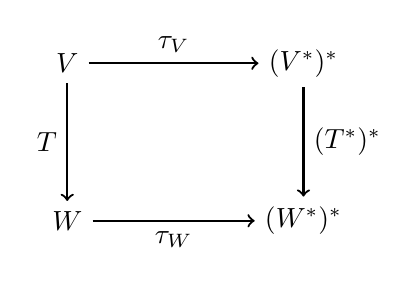
\begin{tikzpicture}[node distance=3cm, auto, thick]
    \node (V) {$V$};
    \node (Vdual) [right of=V] {$(V^*)^*$};
    \node (W) [below of=V, node distance=2cm] {$W$};
    \node (Wdual) [right of=W] {$(W^*)^*$};

    \draw[->] (V) to node {$\tau_V$} (Vdual);
    \draw[->] (V) to node[swap] {$T$} (W);
    \draw[->] (W) to node[swap] {$\tau_W$} (Wdual);
    \draw[->] (Vdual) to node {$(T^*)^*$} (Wdual);
  \end{tikzpicture}
\end{center}
% Creator: Opus 5
In other words, $(T^*)^* \circ \tau_V = \tau_W \circ T$.
\end{proposition*}

\begin{proof}
Both sides are maps $V \to (W^*)^*$, so it is enough to compare their values at an arbitrary $v \in V$; those values are functionals on $W^*$, so it is enough in turn to compare them at an arbitrary $\ell \in W^*$. Unwinding the definition of the dual map, \cref{lem:dual_map}, twice, and that of $\tau$, which is the same formula for every space,
\begin{align*}
\Big( (T^*)^*\big(\tau_V(v)\big) \Big)(\ell)
  &= \big(\tau_V(v) \circ T^*\big)(\ell) = \tau_V(v)\big(T^*(\ell)\big) = \big(T^*(\ell)\big)(v) \\
  &= (\ell \circ T)(v) = \ell\big(T(v)\big) = \tau_W\big(T(v)\big)(\ell).
\end{align*}
Hence $(T^*)^*(\tau_V(v)) = \tau_W(T(v))$ for every $v \in V$, which is precisely the commutativity of the square. Note that nothing here requires $V$ or $W$ to be finite-di\-men\-sional.
\end{proof}
% Extractor: Gemini 3.1 Pro

\begin{exercise}[Canonical Evaluation on Dual Bases]
  \label{exc:tau_on_dual_bases}
  Let $V$ be a finite-di\-men\-sional vector space over $K$, and let $\mathcal{B} = (v_1, \dots, v_n)$ be a basis for $V$. Let $\mathcal{B}^* = (v_1^*, \dots, v_n^*)$ be the dual basis, and let $(\mathcal{B}^*)^* = ((v_1^*)^*, \dots, (v_n^*)^*)$ be the basis for $(V^*)^*$ which is dual to $\mathcal{B}^*$. Show that $\tau(\mathcal{B}) = (\mathcal{B}^*)^*$, meaning $\tau(v_i) = (v_i^*)^*$ for all $1 \leq i \leq n$.
  \exinfo{This exercise is Problem 2 of Problem Sheet 14, Linear Algebra I, Autumn Semester 2025.}
\end{exercise}

\begin{exercise}[Every Finite-Dimensional Space is a Dual Space]
\label{exc:every_finite_dim_is_dual_sc}
Is every finite-dimensional vector space $V$ over $K$ isomorphic to the dual space of some finite-dimensional vector space?
\begin{enumerate}
    \item True
    \item False
\end{enumerate}
\exinfo{This exercise is Single Choice Question 2 of Problem Sheet 14, Linear Algebra I, Autumn Semester 2025.}
\end{exercise}

% Creator: Opus 5
\subsection{Solutions to the Exercises}
\label{sec:solutions_hom_dual}

\begin{exercisesolution}[Proof of \cref{exc:hom_axioms}]
For the linearity of $\alpha \cdot T$: for $a \in K$ and $v, v' \in V$,
\[
(\alpha T)(a v + v') = \alpha \, T(av + v') = \alpha \big( a T(v) + T(v') \big) = a \cdot \alpha T(v) + \alpha T(v') = a \, (\alpha T)(v) + (\alpha T)(v').
\]

The vector space axioms for $\Hom(V,W)$ all reduce to the corresponding axioms in $W$, because both operations are defined pointwise. For instance, associativity of addition: for all $v \in V$,
\[
\big((T_1 + T_2) + T_3\big)(v) = \big(T_1(v) + T_2(v)\big) + T_3(v) = T_1(v) + \big(T_2(v) + T_3(v)\big) = \big(T_1 + (T_2 + T_3)\big)(v),
\]
using associativity in $W$ in the middle; since two maps agreeing at every $v$ are equal, $(T_1 + T_2) + T_3 = T_1 + (T_2 + T_3)$. The same pattern gives commutativity, $1 \cdot T = T$, $(\alpha\beta) \cdot T = \alpha \cdot (\beta \cdot T)$, and the two distributive laws, the one for $\alpha \cdot (T_1 + T_2)$ is written out in the text above. The additive inverse of $T$ is $(-1) \cdot T$, since $(T + (-1)T)(v) = T(v) - T(v) = 0$ for all $v$.

For the additivity of $\Psi_{\mathcal{C}}^{\mathcal{B}}$: its $j$-th column at $T_1 + T_2$ is
\[
[(T_1 + T_2)(v_j)]_{\mathcal{C}} = [T_1(v_j) + T_2(v_j)]_{\mathcal{C}} = [T_1(v_j)]_{\mathcal{C}} + [T_2(v_j)]_{\mathcal{C}},
\]
because the coordinate map $\Phi_{\mathcal{C}}$ is linear. Columnwise addition of matrices is addition of matrices, so $\Psi_{\mathcal{C}}^{\mathcal{B}}(T_1 + T_2) = \Psi_{\mathcal{C}}^{\mathcal{B}}(T_1) + \Psi_{\mathcal{C}}^{\mathcal{B}}(T_2)$.
\end{exercisesolution}

\begin{exercisesolution}[Proof of \cref{exc:row_space_is_dual}]
Linearity of $D$: for $\ell, \ell' \in K^n_{\text{row}}$, $\alpha \in K$ and every $v \in K^n_{\text{col}}$,
\[
f_{\alpha \ell + \ell'}(v) = (\alpha \ell + \ell') \cdot v = \alpha (\ell \cdot v) + \ell' \cdot v = \alpha f_{\ell}(v) + f_{\ell'}(v),
\]
by the distributivity of matrix multiplication, so $D(\alpha \ell + \ell') = \alpha D(\ell) + D(\ell')$.

Injectivity: if $D(\ell) = 0$, then $\ell \cdot v = 0$ for every $v \in K^n_{\text{col}}$; taking $v = e_i$ picks out the $i$-th entry of $\ell$, so every entry of $\ell$ vanishes and $\ell = 0$. Since $\dim K^n_{\text{row}} = n = \dim K^n_{\text{col}} = \dim (K^n_{\text{col}})^*$ by \cref{cor:dim_dual}, an injective linear map between these two spaces is an isomorphism by \cref{cor:equal_dim_iso}.
\end{exercisesolution}

\begin{exercisesolution}[Proof of \cref{prop:dual_functoriality} and of \cref{exc:dual_functoriality}]
For the composition rule, both $(S \circ T)^*$ and $T^* \circ S^*$ are maps $U^* \to V^*$, so it suffices to evaluate them at an arbitrary $\ell \in U^*$:
\[
(S \circ T)^*(\ell) = \ell \circ (S \circ T) = (\ell \circ S) \circ T = T^*(\ell \circ S) = T^*\big(S^*(\ell)\big) = (T^* \circ S^*)(\ell),
\]
using only the associativity of composition. Hence $(S \circ T)^* = T^* \circ S^*$.

\begin{enumerate}[label=\textbf{(\alph*)}]
    \item For $\ell \in V^*$ we have $(\id_V)^*(\ell) = \ell \circ \id_V = \ell$, so $(\id_V)^* = \id_{V^*}$.
    \item For $\ell \in V^*$ and $v \in V$, $\big(0^*(\ell)\big)(v) = \ell(0(v)) = \ell(0_V) = 0$, so $0^*(\ell)$ is the zero functional for every $\ell$, that is, $0^*$ is the zero map $V^* \to V^*$. \qedhere
\end{enumerate}
\end{exercisesolution}

\begin{exercisesolution}[Proof of \cref{exc:tau_on_dual_bases}]
Both $\tau(v_i)$ and $(v_i^*)^*$ are elements of $(V^*)^*$, that is, functionals on $V^*$. Since $\mathcal{B}^* = (v_1^*, \dots, v_n^*)$ is a basis of $V^*$, it suffices to check that they agree on each $v_j^*$. By the definition of $\tau$,
\[
\tau(v_i)(v_j^*) = v_j^*(v_i) = \delta_{ji} = \delta_{ij},
\]
while by the definition of the basis dual to $\mathcal{B}^*$,
\[
(v_i^*)^*(v_j^*) = \delta_{ij}.
\]
The two agree on every member of a basis of $V^*$, hence $\tau(v_i) = (v_i^*)^*$ for all $i$, that is, $\tau(\mathcal{B}) = (\mathcal{B}^*)^*$.
\end{exercisesolution}

% Extractor: Gemini 3.1 Pro
\setcounter{section}{1}
\renewcommand{\thetheorem}{18.b.\arabic{theorem}}
\setcounter{theorem}{0}
\section{Direct Sums}

\subsection{The External Direct Sum}

% prop:18.b.1
\begin{proposition}[Vector Space Structure of the Cartesian Product]
  \label{prop:direct_sum_structure}
  Let $V$ and $W$ be two vector spaces over $K$. Then, the Cartesian product $V \times W$ becomes a vector space over $K$, provided we endow it with the following operations:
  \begin{itemize}
    \item $(v_1, w_1) + (v_2, w_2) := (v_1 + v_2, w_1 + w_2)$ for all $(v_1, w_1), (v_2, w_2) \in V \times W$.
    \item $\alpha \cdot (v, w) := (\alpha v, \alpha w)$ for all $\alpha \in K$ and $(v, w) \in V \times W$.
  \end{itemize}
  The zero element of this space is given by $0_{V \times W} := (0_V, 0_W)$. This new vector space $V \times W$ is usually denoted by $V \oplus W$ and is called the direct sum of $V$ and $W$.
\end{proposition}

% Extractor: Opus 5
\begin{exercise}[The Axioms for $V \oplus W$, and the Canonical Maps]
  \label{exc:direct_sum_axioms}
  Verify that all vector space axioms are satisfied by $V \times W$ under the componentwise operations above, so that \cref{prop:direct_sum_structure} holds. Check also that the four canonical maps of the following remark are linear, that $p_V$ and $p_W$ are surjective, and that $i_V$ and $i_W$ are injective.
\end{exercise}

% Extractor: Gemini 3.1 Pro

\begin{remark}[Canonical Maps associated with Direct Sums]
  The direct sum $V \oplus W$ is naturally equipped with several canonical linear maps:
  \begin{enumerate}
    \item \textbf{Canonical Embeddings}:
    \begin{itemize}
      \item $i_V \colon V \to V \oplus W$ defined by $i_V(v) := (v, 0)$.
      \item $i_W \colon W \to V \oplus W$ defined by $i_W(w) := (0, w)$.
    \end{itemize}
    \item \textbf{Canonical Projections}:
    \begin{itemize}
      \item $p_V \colon V \oplus W \to V$ defined by $p_V(v, w) := v$.
      \item $p_W \colon V \oplus W \to W$ defined by $p_W(v, w) := w$.
    \end{itemize}
  \end{enumerate}
  Clearly, all these maps are linear. Furthermore, the projections $p_V$ and $p_W$ are surjective, while the embeddings $i_V$ and $i_W$ are injective. By virtue of these embeddings, we can often identify $V$ and $W$ as subspaces of $V \oplus W$ through the identifications $v \leftrightarrow (v, 0)$ and $w \leftrightarrow (0, w)$.
\end{remark}

\subsection{Internal Direct Sums and Complements}

% prop:18.b.2
\begin{proposition}[Isomorphism to a Complementary Subspace]
  \label{prop:direct_sum_complement}
  Let $V$ be a vector space over $K$, and let $U \subseteq V$ be a subspace. Suppose $U' \subseteq V$ is another subspace that acts as a complement of $U$ in $V$, which by \cref{def:complement} means that $U + U' = V$ and $U \cap U' = \{0\}$. Then, the map
  \[
  \varphi \colon U \oplus U' \to V, \quad \varphi(u, u') := u + u'
  \]
  is a linear isomorphism.
\end{proposition}

\begin{proof}
  The linearity of $\varphi$ follows immediately from the definitions of the operations in $U \oplus U'$ and the linearity of addition in $V$.

  To establish injectivity, suppose $\varphi(u, u') = 0$, which implies $u + u' = 0$, and therefore $u = -u'$. Since $u \in U$ and $u' \in U'$, it follows that $u = -u' \in U \cap U'$. However, as $U'$ is a complement of $U$, we have $U \cap U' = \{0\}$ by definition. Consequently, $u = u' = 0$, which shows that $\ker(\varphi) = \{0_{U \oplus U'}\}$. Thus, $\varphi$ is injective.

  Regarding surjectivity, we observe that since $U'$ is a complement of $U$ in $V$, we have $U + U' = V$ by definition. Thus, for any $v \in V$, there exist $u \in U$ and $u' \in U'$ such that $u + u' = v$. This implies $\varphi(u, u') = v$, and therefore $\Img(\varphi) = V$. This proves that $\varphi$ is surjective, and consequently, an isomorphism.
\end{proof}

\begin{remark}
  While $U \oplus U'$ is formally a different vector space from $V$, the existence of the canonical isomorphism $\varphi$ allows us to treat $V$ as the direct sum of its internal subspaces whenever a complement is specified.
\end{remark}

Geometrically, in $\mathbb{R}^2$, this represents the decomposition of any vector $v$ uniquely into a sum of a vector $u \in U$ and a vector $u' \in U'$, constructed via a parallelogram parallel to the complementary subspaces.

\begin{center}
  \begin{tikzpicture}[scale=1.2]
    % Axes/Subspaces
    \draw[thick, blue] (-2,-1) -- (3,1.5) node[right] {$U$}; % Line U
    \draw[thick, red] (-1,2) -- (1.5,-3) node[right] {$U'$}; % Line U'

    % Vectors
    \draw[->, thick, blue!60!black] (0,0) -- (1.6,0.8) node[midway, above left] {$u$}; % Vector u in U
    \draw[->, thick, red!60!black] (0,0) -- (0.5,-1) node[midway, left] {$u'$}; % Vector u' in U'

    % Parallelogram and Resultant
    \draw[dashed, gray] (1.6,0.8) -- (2.1,-0.2); % Parallel line for parallelogram
    \draw[dashed, gray] (0.5,-1) -- (2.1,-0.2); % Parallel line for parallelogram
    \draw[->, very thick, purple] (0,0) -- (2.1,-0.2) node[right] {$v = u + u'$}; % Resultant vector v

    % Origin
    \filldraw (0,0) circle (1.5pt) node[above left] {$0$};
  \end{tikzpicture}
\end{center}

Similarly, we can extend this intuition to $\mathbb{R}^3$. Consider $U$ to be the $z$-axis (a line through the origin) and $U'$ to be the $xy$-plane (a plane through the origin). Then $U$ and $U'$ are subspaces of $\mathbb{R}^3$.
\begin{itemize}
  \item $U = \Sp(e_3) = \{(0,0,z) \mid z \in \mathbb{R}\}$
  \item $U' = \Sp(e_1, e_2) = \{(x,y,0) \mid x,y \in \mathbb{R}\}$
\end{itemize}
Any vector $v = (x,y,z) \in \mathbb{R}^3$ can be uniquely written as a sum of a vector $u \in U$ and a vector $u' \in U'$:
$v = (0,0,z) + (x,y,0)$.
Here, $u = (0,0,z) \in U$ and $u' = (x,y,0) \in U'$.
Furthermore, $U \cap U' = \{(0,0,0)\}$, which is the zero vector.
Thus, $\mathbb{R}^3 = U \oplus U'$. Geometrically, this means any point in 3D space can be reached by first moving along the $z$-axis and then moving in the $xy$-plane.

\begin{center}
  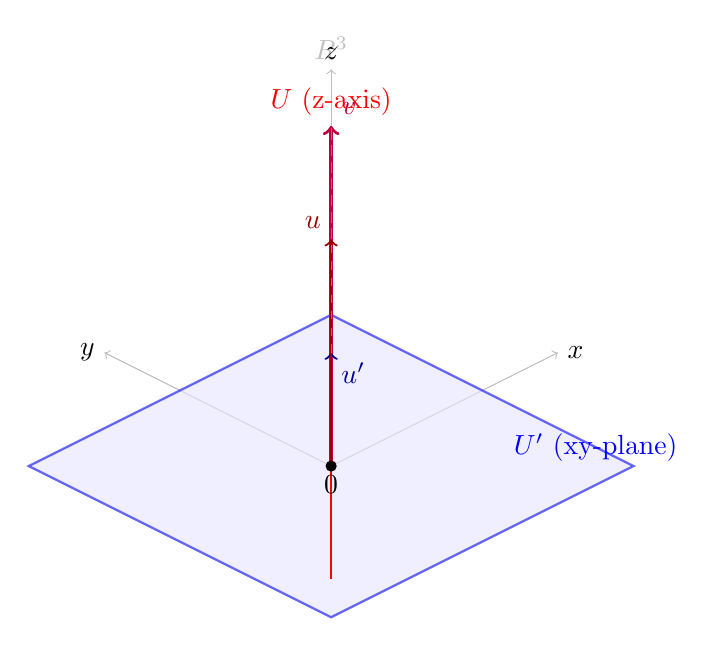
\begin{tikzpicture}[scale=1.2, x={(0.8cm,0.4cm)}, y={(-0.8cm,0.4cm)}, z={(0cm,1.2cm)}]
    % Coordinate axes
    \draw[->, gray!50] (0,0,0) -- (3,0,0);
    \draw[->, gray!50] (0,0,0) -- (0,3,0);
    \draw[->, gray!50] (0,0,0) -- (0,0,3.5) node[above] {$\mathbb{R}^3$};
    \node[right] at (3,0,0) {$x$};
    \node[left] at (0,3,0) {$y$};
    \node[above] at (0,0,3.5) {$z$};

    % The subspace U' (xy-plane)
    \filldraw[blue!10, draw=blue, thick, opacity=0.6] (-2,-2,0) -- (2,-2,0) -- (2,2,0) -- (-2,2,0) -- cycle; % xy-plane
    \node[blue] at (2, -1.5, 0) {$U'$ (xy-plane)};

    % The subspace U (z-axis)
    \draw[thick, red] (0,0,-1) -- (0,0,3) node[above] {$U$ (z-axis)}; % z-axis

    % A vector v
    \coordinate (v_coord) at (1.5, 1.5, 2);
    \draw[->, very thick, purple] (0,0,0) -- (v_coord) node[above right] {$v$};

    % Decomposition of v
    \coordinate (u_prime_coord) at (1.5, 1.5, 0);
    \coordinate (u_coord) at (0, 0, 2);
    \draw[->, thick, blue!60!black] (0,0,0) -- (u_prime_coord) node[below right] {$u'$};
    \draw[->, thick, red!60!black] (0,0,0) -- (u_coord) node[above left] {$u$};
    \draw[dashed, gray] (u_prime_coord) -- (v_coord);
    \draw[dashed, gray] (u_coord) -- (v_coord);
    \filldraw (0,0,0) circle (1.5pt) node[below] {$0$};
  \end{tikzpicture}
\end{center}

\subsection{Generalization to Multiple Summands}

The concept of a direct sum can be extended to any finite collection of vector spaces $U_1, \dots, U_m$ over $K$. We define their direct sum as:
\[
U_1 \oplus \dots \oplus U_m := U_1 \times \dots \times U_m,
\]
endowed with coordinatewise operations.

For an infinite family of vector spaces $\{U_i\}_{i \in I}$, we define the direct sum $\bigoplus_{i \in I} U_i$ as the set of functions $t \colon I \to \bigcup_{i \in I} U_i$ such that $t(i) \in U_i$ for all $i \in I$, and $t(i) \neq 0$ for at most finitely many indices $i \in I$. This ensures that any element of the direct sum can be represented as a finite formal sum of components.

% Creator: Opus 5
\subsection{Solutions to the Exercises}
\label{sec:solutions_direct_sums}

\begin{exercisesolution}[Proof of \cref{exc:direct_sum_axioms}]
Every axiom for $V \times W$ is checked coordinatewise and reduces to the same axiom in $V$ and in $W$. For instance, for $(v_1,w_1), (v_2,w_2), (v_3,w_3) \in V \times W$,
\[
\big((v_1,w_1) + (v_2,w_2)\big) + (v_3,w_3) = (v_1 + v_2 + v_3, \; w_1 + w_2 + w_3) = (v_1,w_1) + \big((v_2,w_2) + (v_3,w_3)\big),
\]
using associativity in $V$ in the first coordinate and in $W$ in the second. The same pattern gives commutativity, the neutral element $(0_V, 0_W)$, the additive inverse $-(v,w) = (-v,-w)$, and the four axioms involving scalars, for instance $\alpha \cdot \big((v_1,w_1) + (v_2,w_2)\big) = (\alpha v_1 + \alpha v_2, \alpha w_1 + \alpha w_2) = \alpha (v_1,w_1) + \alpha (v_2,w_2)$.

The canonical maps are linear for the same reason: $i_V(\alpha v + v') = (\alpha v + v', 0) = \alpha (v,0) + (v',0) = \alpha \, i_V(v) + i_V(v')$, and
\[
p_V\big(\alpha (v,w) + (v',w')\big) = p_V(\alpha v + v', \; \alpha w + w') = \alpha v + v' = \alpha \, p_V(v,w) + p_V(v',w'),
\]
and symmetrically for $i_W$ and $p_W$.

The projections are surjective, since $p_V(v, 0) = v$ for every $v \in V$ and $p_W(0,w) = w$ for every $w \in W$. The embeddings are injective, since $i_V(v) = (v,0) = (0,0)$ forces $v = 0$, so $\ker(i_V) = \{0\}$, and likewise for $i_W$.
\end{exercisesolution}

% Extractor: Gemini 3.1 Pro

\setcounter{section}{2}
\renewcommand{\thetheorem}{18.c.\arabic{theorem}}
\setcounter{theorem}{0}
\section{Quotient Spaces}

\subsection{Equivalence Relation and the Quotient Space}

Let $V$ be a vector space over $K$, and let $U \subseteq V$ be a subspace. We will define a new vector space over $K$, denoted by $V/U$, together with a linear map $\pi \colon V \to V/U$ such that $\pi$ is surjective and $\ker(\pi) = U$. The space $V/U$ will have some other good properties. The space $V/U$ will be called the \newterm{quotient} of $V$ by $U$, or $V$ modulo $U$, and the map $\pi$ the \newterm{quotient map}, or the \newterm{projection onto the quotient space}.

We begin by defining a relation on $V$. For $v_1, v_2 \in V$, we define $v_1 \sim v_2$ if and only if $v_1 - v_2 \in U$.

\begin{lemma*}[Equivalence Relation on $V$]
\label{lem:quotient_equivalence_relation}
  The relation $\sim$ defines an equivalence relation on $V$.
\end{lemma*}

\begin{proof}
  Reflexivity: For all $v \in V$, $v \sim v$ because $v - v = 0 \in U$.

  Symmetry: If $v_1 \sim v_2$, then $v_1 - v_2 \in U$. Since $U$ is a subspace, $-(v_1 - v_2) = v_2 - v_1 \in U$, which implies $v_2 \sim v_1$.

  Transitivity: If $v_1 \sim v_2$ and $v_2 \sim v_3$, then $v_1 - v_2 \in U$ and $v_2 - v_3 \in U$. Because $U$ is a subspace, their sum is in $U$:
  \[ (v_1 - v_2) + (v_2 - v_3) = v_1 - v_3 \in U, \]
  which means $v_1 \sim v_3$.
\end{proof}

We denote the equivalence class of $v \in V$ by $[v]$. Thus,
\[ [v] = v + U = \{v + u \mid u \in U\}. \]

% def:18.c.1
\begin{definition}[The Quotient Space]
  \label{def:quotient_space}
  Let $V$ be a vector space over $K$, and let $U \subseteq V$ be a subspace. We define $V/U := V/\sim$ to be the set of equivalence classes of the equivalence relation $\sim$, which is one by the Lemma on \cpageref{lem:quotient_equivalence_relation}. So, the elements of $V/U$ are $[v]$, where $v \in V$.
  
  Alternatively, each element in $V/U$ is a set of the form $v + U$, where $v \in V$. The space $V/U$ is called the quotient of $V$ by $U$ (or modulo $U$).
\end{definition}
\bigbreak
Geometrically, the nature of the quotient space $\mathbb{R}^2/U$ depends on the dimension of $U$:
\begin{itemize}
  \item If $U = \{0\}$ is the trivial subspace, then each equivalence class $[v] = v + \{0\} = \{v\}$ is simply a single \textbf{point}. In this case, no points are \qt{collapsed} together, and therefore $\mathbb{R}^2/\{0\} \cong \mathbb{R}^2$.
  \item If $U$ is a \textbf{line} through the origin, the equivalence classes $[v]$ forming the space $\mathbb{R}^2/U$ are the lines parallel to $U$, as seen in \cref{fig:quotient_r2}.
\end{itemize}

\begin{figure}[ht!]
  \centering
  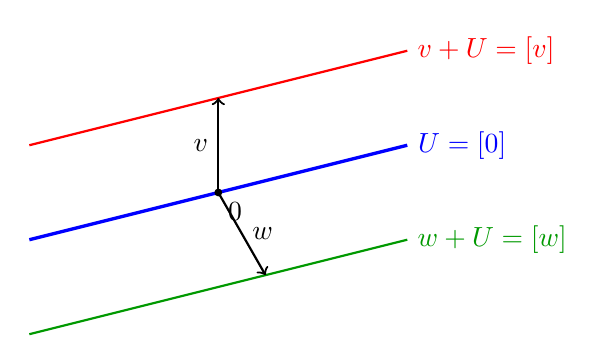
\begin{tikzpicture}[scale=0.6]
    % The subspace U (origin line)
    \draw[very thick, blue] (-4,-1) -- (4,1) node[right] {$U = [0]$};

    % Other equivalence classes (Cosets)
    \draw[thick, red] (-4, 1) -- (4, 3) node[right] {$v + U = [v]$};
    \draw[thick, green!60!black] (-4, -3) -- (4, -1) node[right] {$w + U = [w]$};

    % Vectors defining the shift
    \draw[->, thick] (0,0) -- (0,2) node[midway, left] {$v$};
    \draw[->, thick] (0,0) -- (1,-1.75) node[midway, right] {$w$};

    % Origin
    \filldraw (0,0) circle (2pt) node[below right] {$0$};
  \end{tikzpicture}
  \caption{Geometric interpretation of the quotient space $\mathbb{R}^2/U$.}
  \label{fig:quotient_r2}
\end{figure}

Similarly, we can extend this intuition to $\mathbb{R}^3$, as illustrated in \cref{fig:quotient_r3}:
\begin{itemize}
  \item If $U = \{0\}$ is the trivial subspace, then each equivalence class $[v] = \{v\}$ is simply a \textbf{point}. Since no two distinct vectors are identified, the quotient space $\mathbb{R}^3/\{0\}$ is isomorphic to $\mathbb{R}^3$ itself.
  \item If $U$ is a \textbf{plane} through the origin, then $\mathbb{R}^3/U$ is 1-dimensional (by \cref{prop:dim_quotient}) and therefore isomorphic to a line. Each element $[v]$ is a plane parallel to $U$. The quotient space can be viewed as the set of all such parallel planes \qt{stacked} along a transversal direction (see \cref{fig:quotient_plane} and \cref{prop:iso_complement}).
  \item If $U$ is a \textbf{line} through the origin, then $\mathbb{R}^3/U$ is 2-dimensional (by \cref{prop:dim_quotient}) and therefore isomorphic to a plane. Each element $[v]$ is a line parallel to $U$ (see \cref{fig:quotient_line} and \cref{prop:iso_complement}).
  \item If $U = \mathbb{R}^3$ is the entire space, then there is only one equivalence class, $[v] = \mathbb{R}^3$. The quotient space $\mathbb{R}^3/\mathbb{R}^3$ is the zero vector space, with dimension $0$.
\end{itemize}

\begin{remark}
  The crucial insight is that an equivalence class $[v] = v + U = \{v + u \mid u \in U\}$ is not merely a single vector, but a translate of the subspace $U$. Consequently, the ``shape'' or dimension of $[v]$ is identical to the dimension of $U$. Specifically:
  \begin{itemize}
    \item If $U$ is a line, then every $[v]$ is a line parallel to $U$.
    \item If $U$ is a plane, then every $[v]$ is a plane parallel to $U$.
  \end{itemize}
  The dimension of the quotient space $V/U$ represents the number of independent directions available to shift these objects. For instance, in $\mathbb{R}^3$, if $U$ is a line (1-dimensional), there are 2 independent directions in which one can move this line to obtain a distinct parallel line (effectively moving the line across a 2-dimensional plane). 
  
  Thus, the space of all such lines is 2-dimensional. This geometric intuition aligns perfectly with the dimension formula established in \cref{prop:dim_quotient}. In the case where $U = \{0\}$, the equivalence class is a point (0-dimensional), and we retain all 3 degrees of freedom of the ambient space.
\end{remark}

\begin{figure}[h!]
  \centering
  \begin{subfigure}[b]{0.31\textwidth}
    \centering
    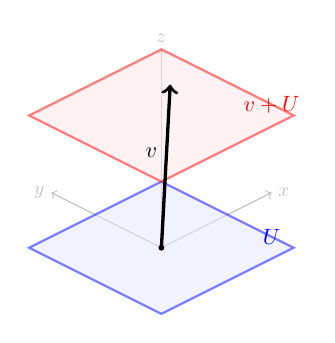
\begin{tikzpicture}[scale=0.7, x={(0.8cm,0.4cm)}, y={(-0.8cm,0.4cm)}, z={(0cm,1.2cm)}]
      % Plane Case
      \draw[->, gray!50] (0,0,0) -- (2.5,0,0) node[right, scale=0.7] {$x$};
      \draw[->, gray!50] (0,0,0) -- (0,2.5,0) node[left, scale=0.7] {$y$};
      \draw[->, gray!50] (0,0,0) -- (0,0,3) node[above, scale=0.7] {$z$};
      \filldraw[blue!10, draw=blue, thick, opacity=0.5] (-1.5,-1.5,0) -- (1.5,-1.5,0) -- (1.5,1.5,0) -- (-1.5,1.5,0) -- cycle;
      \node[blue, scale=0.8] at (1.5, -1, 0) {$U$};
      \filldraw[red!10, draw=red, thick, opacity=0.5] (-1.5,-1.5,2) -- (1.5,-1.5,2) -- (1.5,1.5,2) -- (-1.5,1.5,2) -- cycle;
      \node[red, scale=0.8] at (1.5, -1, 2) {$v + U$};
      \draw[->, very thick, black] (0,0,0) -- (0.8,0.6,2) node[midway, above left, scale=0.8] {$v$};
      \filldraw (0,0,0) circle (1.2pt);
    \end{tikzpicture}
    \caption{Plane case ($1D$-quotient)}
    \label{fig:quotient_plane}
  \end{subfigure}%
  \hspace{1cm}%
  \begin{subfigure}[b]{0.31\textwidth}
    \centering
    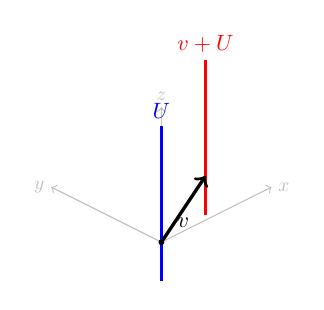
\begin{tikzpicture}[scale=0.7, x={(0.8cm,0.4cm)}, y={(-0.8cm,0.4cm)}, z={(0cm,0.7cm)}]
      % Line Case (Shorter Z)
      \draw[->, gray!50] (0,0,0) -- (2.5,0,0) node[right, scale=0.7] {$x$};
      \draw[->, gray!50] (0,0,0) -- (0,2.5,0) node[left, scale=0.7] {$y$};
      \draw[->, gray!50] (0,0,0) -- (0,0,3.5) node[above, scale=0.7] {$z$};
      \draw[thick, blue] (0,0,-1) -- (0,0,3) node[above, scale=0.8] {$U$};
      \draw[thick, red] (2,1,-1) -- (2,1,3) node[above, scale=0.8] {$v + U$};
      % Vector v in foreground
      \draw[->, very thick, black] (0,0,0) -- (2,1,0) node[midway, below, scale=0.8] {$v$};
      \filldraw (0,0,0) circle (1.2pt);
    \end{tikzpicture}
    \caption{Line case ($2D$-quotient)}
    \label{fig:quotient_line}
  \end{subfigure}
  \caption{Geometric interpretation of the quotient space $\mathbb{R}^3/U$.}
  \label{fig:quotient_r3}
\end{figure}

\subsection{The Vector Space Structure of \texorpdfstring{$V/U$}{V/U}}

We want to turn $V/U$ into a vector space over $K$. We define addition as $[v_1] + [v_2] := [v_1 + v_2]$ for all $[v_1], [v_2] \in V/U$. Alternatively, this can be written as $(v_1 + U) + (v_2 + U) := (v_1 + v_2) + U$. For scalar multiplication, let $\alpha \in K$ and $[v] \in V/U$. We define $\alpha \cdot [v] := [\alpha v]$. The zero element is defined as $0_{V/U} := [0_V] = U$.

% prop:18.c.2
\begin{proposition}[Well-definedness of Operations in $V/U$]
  \label{prop:quotient_operations}
  The operations defined above are well-defined. Moreover, they give $V/U$ the structure of a vector space over $K$.
\end{proposition}

\begin{proof}
  To establish well-definedness, we must show that the operations do not depend on the choice of representatives.
  For scalar multiplication, suppose $[v] = [v']$, and let $\alpha \in K$. We need to show that $[\alpha v] = [\alpha v']$. Indeed, since $[v] = [v']$, we have $v - v' \in U$. Because $U$ is a subspace, $\alpha(v - v') = \alpha v - \alpha v' \in U$. Consequently, $[\alpha v] = [\alpha v']$.

  Similarly, for addition, suppose $[v_1] = [v_1']$ and $[v_2] = [v_2']$. We need to show that $[v_1 + v_2] = [v_1' + v_2']$. By assumption, $v_1 - v_1' \in U$ and $v_2 - v_2' \in U$. Adding these yields:
  \[ (v_1 + v_2) - (v_1' + v_2') = (v_1 - v_1') + (v_2 - v_2') \in U. \]
  Therefore, $v_1 + v_2 \sim v_1' + v_2'$, which implies $[v_1 + v_2] = [v_1' + v_2']$. This proves that the operations are well-defined.

  It remains to show that they satisfy the axioms of a vector space. These follow directly from the corresponding axioms in $V$; the notes leave that verification to the reader, and it is carried out among the solutions at the end of this section.
\end{proof}

% Extractor: Opus 5
\begin{exercise}[The Axioms for $V/U$]
  \label{exc:quotient_axioms}
  Complete the proof of \cref{prop:quotient_operations} by checking that the operations on $V/U$ satisfy the axioms of a vector space.
\end{exercise}

% Extractor: Gemini 3.1 Pro

We now define a map $\pi \colon V \to V/U$ by $\pi(v) := [v] \in V/U$ for all $v \in V$.

% prop:18.c.3
\begin{proposition}[The Quotient Map]
  \label{prop:quotient_map}
  The map $\pi \colon V \to V/U$ is a linear map. Moreover, it is surjective (i.e., $\Img(\pi) = V/U$), and $\ker(\pi) = U$.
\end{proposition}

\begin{proof}
  Linearity: For $v_1, v_2 \in V$, $\pi(v_1 + v_2) = [v_1 + v_2] = [v_1] + [v_2] = \pi(v_1) + \pi(v_2)$. For $\alpha \in K$ and $v \in V$, $\pi(\alpha v) = [\alpha v] = \alpha [v] = \alpha \pi(v)$.

  Surjectivity: Let $x \in V/U$. By definition, $x$ is an equivalence class $[v]$ of some element $v \in V$. Thus, $x = \pi(v)$.

  Kernel: We claim that $\ker(\pi) = U$. First, let $v \in \ker(\pi)$, meaning $\pi(v) = 0$. Then, $[v] = [0]$, which implies $v = v - 0 \in U$. Hence, $\ker(\pi) \subseteq U$. Conversely, let $u \in U$. Then, $u \sim 0$ because $u - 0 \in U$. Therefore, $\pi(u) = [u] = [0] = 0$, so $u \in \ker(\pi)$. This shows that $U \subseteq \ker(\pi)$, completing the proof.
\end{proof}

\begin{proposition}[Dimension of the Quotient Space]
% prop:18.c.4
  \label{prop:dim_quotient}
  Suppose that $V$ is a finite-dimensional vector space. Then, $V/U$ is also finite-dimensional, and $\dim V/U = \dim V - \dim U$.
\end{proposition}

\begin{proof}
  We have seen that $\pi \colon V \to V/U$ is a surjective linear map, this being \cref{prop:quotient_map}. This guarantees that $V/U$ is finite-dimensional. (Generally, if $T \colon W' \to W''$ is a surjective linear map and $W'$ is finite-dimensional, then $W''$ is also finite-dimensional, because the images of a basis of $W'$ span $W''$).

  We now apply the Rank-Nullity Theorem, \cref{thm:rank_nullity}, to $\pi$:
  \[ \dim V = \dim \ker(\pi) + \dim \Img(\pi). \]
  Since $\ker(\pi) = U$ and $\Img(\pi) = V/U$, again by \cref{prop:quotient_map}, we obtain $\dim V/U = \dim V - \dim U$.
\end{proof}

\subsection{The Isomorphism Theorem and Universal Property}

% thm:18.c.5
\begin{theorem}[The First Isomorphism Theorem]
  \label{thm:first_isomorphism}
  Let $V$ and $W$ be vector spaces over $K$, and let $T \colon V \to W$ be a linear map. We define a new map $\overline{T} \colon V/\ker(T) \to \Img(T)$ as follows: For $x \in V/\ker(T)$, choose a representative $v \in V$ such that $x = [v]$. Define $\overline{T}(x) := T(v)$. Then:
  \begin{enumerate}
    \item $\overline{T}$ is well-defined and is a linear map.
    \item $\overline{T} \colon V/\ker(T) \to \Img(T)$ is an isomorphism.
    \item {The following diagram commutes: $T = i \circ \overline{T} \circ \pi$, where $i \colon \Img(T) \to W$ is the inclusion map.
      \begin{center}
        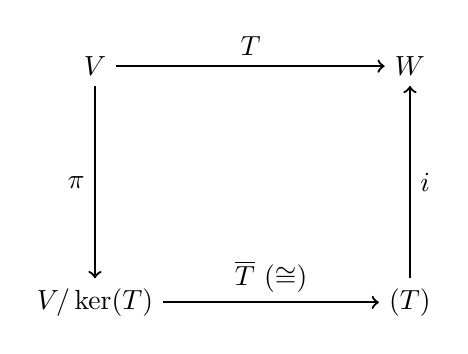
\begin{tikzpicture}[node distance=3cm, auto, thick]
          \node (V) {$V$};
          \node (W) [right of=V, node distance=4cm] {$W$};
          \node (Vmod) [below of=V] {$V/\ker(T)$};
          \node (Im) [below of=W] {$\Img(T)$};

          \draw[->] (V) to node {$T$} (W);
          \draw[->] (V) to node[swap] {$\pi$} (Vmod);
          \draw[->] (Vmod) to node {$\overline{T} \ (\cong)$} (Im);
          \draw[->] (Im) to node[swap] {$i$} (W);
        \end{tikzpicture}
      \end{center}
    }

  \end{enumerate}
\end{theorem}

\begin{proof}
  \begin{enumerate}
    \item To show that $\overline{T}$ is well-defined, suppose $x = [v] = [v']$. We must show that $T(v) = T(v')$. Indeed, $[v] = [v']$ implies that $v - v' \in \ker(T)$, meaning $T(v - v') = 0$. By linearity, $T(v) = T(v')$.

    The linearity of $\overline{T}$ is straightforward: $\overline{T}(\alpha[v]) = \overline{T}([\alpha v]) = T(\alpha v) = \alpha T(v) = \alpha \overline{T}([v])$. Also, $\overline{T}([v_1] + [v_2]) = \overline{T}([v_1 + v_2]) = T(v_1 + v_2) = T(v_1) + T(v_2) = \overline{T}([v_1]) + \overline{T}([v_2])$.

    \item To show that $\overline{T}$ is injective, let $x \in \ker(\overline{T})$, and write $x = [v]$ for some $v \in V$. Then, $\overline{T}(x) = T(v) = 0$, meaning $v \in \ker(T)$. This implies that $x = [v] = 0_{V/\ker(T)}$.

    To show that $\overline{T}$ is surjective, let $w \in \Img(T)$. Then, there exists $v \in V$ such that $T(v) = w$. Consequently, $\overline{T}([v]) = T(v) = w$, proving surjectivity.

    \item The commutativity of the diagram follows immediately from the definitions; the notes leave this to the reader, and it is checked among the solutions at the end of this section.
  \end{enumerate}
\end{proof}

% Extractor: Opus 5
\begin{exercise}[Commutativity of the Diagram in \cref{thm:first_isomorphism}]
  \label{exc:first_iso_diagram}
  Check that $T = i \circ \overline{T} \circ \pi$, where $i \colon \Img(T) \to W$ is the inclusion.
\end{exercise}

% Extractor: Gemini 3.1 Pro

\begin{theorem}[Universal Property of Quotient Spaces]
% thm:18.c.6
  \label{thm:universal_property_quotient}
  Let $V$ be a vector space over $K$, and let $U \subseteq V$ be a subspace. The quotient space $V/U$ has the following universal property: For every vector space $W$ and every linear map $T \colon V \to W$ for which $T(U) = 0$ (i.e., for which $\ker(T) \supseteq U$), there exists a unique linear map $T' \colon V/U \to W$ such that $T = T' \circ \pi$. Moreover, $\ker(T') = \ker(T)/U$.
\end{theorem}

\begin{remark}
  In algebraic jargon, every linear map $T \colon V \to W$ that maps $U$ to $0$ factors through $V/U$ via $T = T' \circ \pi$, and moreover, in a unique way. We say that $T$ induces the map $T'$, or that $T$ descends to a map $T' \colon V/U \to W$.
\end{remark}

\begin{proof}
  We define $T' \colon V/U \to W$ as follows: let $x \in V/U$. Choose $v \in V$ such that $x = [v]$. Define $T'(x) := T(v)$.

  \begin{exercise}[Well-definedness and Linearity of the Induced Map]
    \label{exc:induced_map_well_defined}
    \begin{enumerate}[label=\textbf{(\alph*)}]
      \item Show that $T'$ is well-defined (i.e., if $[v] = [v']$, then $T(v) = T(v')$).
      \item Show that $T'$ is linear.
    \end{enumerate}
  \end{exercise}

  The diagram commutes by construction, since for all $v \in V$, $T' \circ \pi(v) = T'([v]) = T(v)$.

  For uniqueness, suppose $T = T'' \circ \pi$ is another factorization. We will show that $T'' = T'$. Let $x \in V/U$. Since $\pi$ is surjective, there exists $v \in V$ such that $x = \pi(v)$. We then have $T(v) = T'(\pi(v))$ and $T(v) = T''(\pi(v))$, which immediately yields $T'(x) = T''(x)$.
\end{proof}

\begin{exercise}[Kernel of the Induced Quotient Map]
  \label{exc:kernel_induced_map}
  Prove that $\ker(T') = \ker(T)/U$.
\end{exercise}

\subsection{Quotients, Complements, and Dual Spaces}

Let $V$ be a vector space over $K$, and let $U \subseteq V$ be a subspace. Let $W \subseteq V$ be a complement of $U$ in the sense of \cref{def:complement} (i.e., $W$ is a subspace such that $U \cap W = \{0\}$ and $U + W = V$).

\begin{proposition}[Canonical Isomorphism from a Complement]
% prop:18.c.7
  \label{prop:iso_complement}
  Under the assumptions above, there is a canonical isomorphism $Q \colon W \to V/U$, defined by $Q(w) := [w] \in V/U$ for all $w \in W$.
\end{proposition}

\begin{remark}
  The isomorphism $Q$ is canonical only once the complement $W$ is specified. In general, there are many choices of complements to $U$, and there is no preferred choice.
\end{remark}

\begin{proof}
  Consider the inclusion map $i \colon W \to V$ and the projection map $\pi \colon V \to V/U$. Since $Q = \pi \circ i$, $Q$ is a linear map.

  We claim that $\ker(Q) = \{0\}$. Indeed, if $w \in \ker(Q)$, then $[w] = 0$, implying that $w \in U$. However, since $w \in W$, we must have $w \in U \cap W = \{0\}$, and therefore $w = 0$. This shows that $\ker(Q) = \{0\}$.

  We also claim that $Q$ is surjective. Let $x \in V/U$ and choose $v \in V$ such that $x = [v]$. Since $V = U + W$, there exist $u \in U$ and $w \in W$ such that $v = w + u$. It follows that $[v] = [w + u] = [w]$, so $Q(w) = x$. This proves that $Q$ is surjective, and consequently, an isomorphism.
\end{proof}

\begin{exercise}[Inverse Isomorphism from a Complement]
  \label{exc:inverse_from_complement}
  Describe the inverse of $Q$, $Q^{-1} \colon V/U \xrightarrow{\cong} W$.
\end{exercise}

\subsection{Quotients, Complements, and Annihilators}

\begin{proposition}[Annihilators and Dual Quotients]
% prop:18.c.8
  \label{prop:annihilator_dual_quotient}
  Let $U \subseteq V$ be a subspace, and define the \newterm{annihilator} $U^\perp := \{\ell \in V^* \mid \ell|_U = 0\}$. Then:
  \begin{enumerate}
    \item $U^\perp \subseteq V^*$ is a linear subspace.
    \item There is a canonical isomorphism $(V/U)^* \cong U^\perp$.
    \item If $V$ is finite-dimensional, then $U^* \cong V^*/U^\perp$.
  \end{enumerate}
\end{proposition}

\begin{proof}
  \begin{enumerate}
    \item Clearly, the zero functional vanishes on $U$. For $\ell_1, \ell_2 \in U^\perp$ and $\alpha, \beta \in K$, we have $(\alpha \ell_1 + \beta \ell_2)(u) = \alpha \ell_1(u) + \beta \ell_2(u) = 0$ for all $u \in U$, establishing that $U^\perp$ is a subspace.

    \item We define a map $L \colon (V/U)^* \to U^\perp$ as follows: Let $S \in (V/U)^*$, i.e., $S \colon V/U \to K$. Define $L(S) \in V^*$ to be $L(S) := S \circ \pi$.

    \begin{exercise}[The Map $L$ Lands in $U^\perp$ and is Linear]
      \label{exc:annihilator_L}
      \begin{enumerate}[label=\textbf{(\alph*)}]
        \item Show that for all $S \in (V/U)^*$, $S \circ \pi \in U^\perp$.
        \item Show that $L$ is a linear map.
      \end{enumerate}
    \end{exercise}
    
    We claim that $L$ is an isomorphism. To see this, we define a map $P \colon U^\perp \to (V/U)^*$ as follows. Let $T \in U^\perp$, i.e., $T \colon V \to K$ such that $T|_U = 0$. By the Universal Property of Quotients, \cref{thm:universal_property_quotient} applied with $W = K$, there exists a unique $T' \colon V/U \to K$ such that $T = T' \circ \pi$. Define $P(T) := T'$.

    We claim that $L \circ P = \id_{U^\perp}$ and $P \circ L = \id_{(V/U)^*}$. Indeed, for all $S \colon V/U \to K$, we have $P \circ L(S) = P(S \circ \pi) = S$, because of the uniqueness statement in \cref{thm:universal_property_quotient}. Also, for all $T \in U^\perp$, $L \circ P(T) = L(T') = T' \circ \pi = T$. This proves that $L$ is bijective, and since we know $L$ is linear, it is an isomorphism. It follows that $P$ is also a linear isomorphism, being the inverse map of the bijective linear map $L$ (\cref{lem:bijective_is_iso}).

    \item Assume $V$ is finite-dimensional. Consider the restriction map $R \colon V^* \to U^*$ defined by $R(\varphi) := \varphi|_U$ for all $\varphi \in V^*$. 

    \begin{exercise}[Linearity of the Restriction Map]
      \label{exc:restriction_linear}
      Show that $R$ is a linear map.
    \end{exercise}

    We claim that $R$ is surjective. Indeed, let $\psi \in U^*$. We need to show that there exists $\varphi \in V^*$ such that $\varphi|_U = \psi$. The finite-dimensionality of $V$ is important here. Pick a basis $u_1, \dots, u_k$ for $U$, and extend it to a basis $u_1, \dots, u_k, v_{k+1}, \dots, v_n$ of $V$, which is possible by the Steinitz Exchange Lemma in the form of \cref{lem:strong_steinitz}. Define a linear map $\varphi \colon V \to K$ by $\varphi(u_i) := \psi(u_i)$ for all $1 \leq i \leq k$, and $\varphi(v_j) := 0$ for all $k < j \leq n$; prescribing the values on a basis in this way does define one and only one linear map, by \cref{thm:existence_uniqueness_linear_map}. Clearly, $\varphi|_U = \psi$ because $\varphi$ and $\psi$ coincide on the elements of a basis of $U$, and two linear maps on $U$ agreeing on a basis of $U$ are equal (the uniqueness half of the same theorem). This proves $\Img(R) = U^*$.

    We claim that $\ker(R) = U^\perp$. Indeed, this follows directly from definitions: $\ker(R) = \{\varphi \in V^* \mid \varphi|_U = 0\} = U^\perp$.
    By the First Isomorphism Theorem, \cref{thm:first_isomorphism} applied to $R$, we get an induced isomorphism $\overline{R} \colon V^*/\ker(R) \to \Img(R)$, which is to say $\overline{R} \colon V^*/U^\perp \xrightarrow{\cong} U^*$.
  \end{enumerate}
\end{proof}

\begin{exercise}[Relationship between Annihilator of Image and Kernel of Dual Map]
  \label{exc:annihilator_image_kernel_dual}
  Let $T \colon V \to W$ be a linear map between vector spaces. Prove that the annihilator of the image of $T$ is equal to the kernel of its dual map:
  \[ (\Img T)^\perp = \ker(T^*). \]
\end{exercise}

% Creator: Opus 5
\subsection{Solutions to the Exercises}
\label{sec:solutions_quotients}

\begin{exercisesolution}[Proof of \cref{exc:quotient_axioms}]
Every axiom is inherited from $V$ by passing to classes. For instance, associativity: for $v_1, v_2, v_3 \in V$,
\[
\big([v_1] + [v_2]\big) + [v_3] = [v_1 + v_2] + [v_3] = [(v_1 + v_2) + v_3] = [v_1 + (v_2 + v_3)] = [v_1] + \big([v_2] + [v_3]\big),
\]
where the middle step is associativity in $V$. Commutativity is identical. The class $[0_V] = U$ is neutral, since $[v] + [0_V] = [v + 0_V] = [v]$, and $[-v]$ is an additive inverse of $[v]$, since $[v] + [-v] = [0_V]$. For scalars, $\alpha([v_1] + [v_2]) = [\alpha(v_1+v_2)] = [\alpha v_1 + \alpha v_2] = \alpha[v_1] + \alpha[v_2]$, and similarly $(\alpha + \beta)[v] = \alpha[v] + \beta[v]$, $(\alpha\beta)[v] = \alpha(\beta[v])$ and $1 \cdot [v] = [v]$. Each of these is the corresponding axiom in $V$ with brackets placed around it, which is legitimate precisely because the operations were shown to be well defined.
\end{exercisesolution}

\begin{exercisesolution}[Proof of \cref{exc:first_iso_diagram}]
Both $T$ and $i \circ \overline{T} \circ \pi$ are maps $V \to W$, so we evaluate at an arbitrary $v \in V$:
\[
\big(i \circ \overline{T} \circ \pi\big)(v) = i\big(\overline{T}([v])\big) = i\big(T(v)\big) = T(v),
\]
using the definition of $\pi$, then the definition of $\overline{T}$ on the class $[v]$ with representative $v$, and finally that $i$ is the inclusion of $\Img(T)$ into $W$.
\end{exercisesolution}

\begin{exercisesolution}[Proof of \cref{exc:induced_map_well_defined}]
\begin{enumerate}[label=\textbf{(\alph*)}]
    \item Suppose $[v] = [v']$. Then $v - v' \in U \subseteq \ker(T)$ by the hypothesis $T(U) = 0$, so $T(v - v') = 0$ and hence $T(v) = T(v')$. So the value $T'([v]) := T(v)$ does not depend on the representative chosen.
    \item For $\alpha \in K$ and $[v], [v'] \in V/U$,
    \[
    T'\big(\alpha [v] + [v']\big) = T'\big([\alpha v + v']\big) = T(\alpha v + v') = \alpha T(v) + T(v') = \alpha \, T'([v]) + T'([v']),
    \]
    using the definition of the operations on $V/U$, then the definition of $T'$, then the linearity of $T$. \qedhere
\end{enumerate}
\end{exercisesolution}

\begin{exercisesolution}[Proof of \cref{exc:kernel_induced_map}]
First note that $\ker(T) \supseteq U$, so the quotient $\ker(T)/U$ makes sense and is a subspace of $V/U$: its elements are the classes $[v]$ with $v \in \ker(T)$.

Let $x \in V/U$ and write $x = [v]$. Then
\[
x \in \ker(T') \iff T'([v]) = 0 \iff T(v) = 0 \iff v \in \ker(T) \iff x \in \ker(T)/U,
\]
where the second step is the definition of $T'$. The middle equivalence is legitimate for either representative of $x$, since $T'$ is well defined. Hence $\ker(T') = \ker(T)/U$.
\end{exercisesolution}

\begin{exercisesolution}[Proof of \cref{exc:inverse_from_complement}]
Let $x \in V/U$. Since $V = U + W$, any representative $v$ of $x$ can be written as $v = u + w$ with $u \in U$ and $w \in W$, and then $x = [v] = [w]$. The map
\[
Q^{-1} \colon V/U \to W, \qquad Q^{-1}(x) := w, \quad \text{where } x = [u + w] \text{ with } u \in U, \, w \in W,
\]
is the inverse of $Q$. It is well defined: if $u + w = u' + w'$ with $u,u' \in U$ and $w,w' \in W$, then $w - w' = u' - u \in U \cap W = \{0\}$, so $w = w'$. And indeed $Q^{-1}(Q(w)) = Q^{-1}([w]) = w$ for $w \in W$, while $Q(Q^{-1}([v])) = Q(w) = [w] = [v]$.

Equivalently, and more compactly: $Q^{-1} = p_W \circ (\text{choice of representative})$, where $p_W$ is the projection of $V = U \oplus W$ onto $W$ furnished by \cref{prop:direct_sum_complement}; the content of the verification above is exactly that this projection is well defined on classes.
\end{exercisesolution}

\begin{exercisesolution}[Proof of \cref{exc:annihilator_L}]
\begin{enumerate}[label=\textbf{(\alph*)}]
    \item Let $S \in (V/U)^*$ and $u \in U$. Then $\pi(u) = [u] = 0_{V/U}$, because $u \in U = \ker(\pi)$, and therefore
    \[
    (S \circ \pi)(u) = S(0_{V/U}) = 0.
    \]
    So $S \circ \pi$ vanishes on $U$, that is, $S \circ \pi \in U^\perp$.
    \item For $S, S' \in (V/U)^*$ and $\alpha \in K$, and every $v \in V$,
    \[
    L(\alpha S + S')(v) = \big((\alpha S + S') \circ \pi\big)(v) = (\alpha S + S')\big(\pi(v)\big) = \alpha \, S(\pi(v)) + S'(\pi(v)) = \big(\alpha L(S) + L(S')\big)(v),
    \]
    so $L(\alpha S + S') = \alpha L(S) + L(S')$. \qedhere
\end{enumerate}
\end{exercisesolution}

\begin{exercisesolution}[Proof of \cref{exc:restriction_linear}]
For $\varphi, \varphi' \in V^*$, $\alpha \in K$ and every $u \in U$,
\[
R(\alpha \varphi + \varphi')(u) = (\alpha \varphi + \varphi')|_U(u) = \alpha \varphi(u) + \varphi'(u) = \big(\alpha R(\varphi) + R(\varphi')\big)(u),
\]
since the operations on $V^*$ are defined pointwise. Two functionals on $U$ agreeing at every $u \in U$ are equal, so $R(\alpha \varphi + \varphi') = \alpha R(\varphi) + R(\varphi')$.
\end{exercisesolution}

\begin{exercisesolution}[Proof of \cref{exc:annihilator_image_kernel_dual}]
Both sides are subsets of $W^*$. For $\ell \in W^*$, the notes' chain of equivalences reads
\[
\ell \in (\Img T)^\perp \iff \ell|_{\Img(T)} = 0 \iff \ell \circ T = 0 \iff T^*(\ell) = 0 \iff \ell \in \ker(T^*).
\]
The middle equivalence is the only one with content: $\ell \circ T$ is the zero map on $V$ exactly when $\ell(T(v)) = 0$ for every $v \in V$, and the values $T(v)$ are precisely the elements of $\Img(T)$, so this says exactly that $\ell$ vanishes on $\Img(T)$. The remaining steps are the definitions of $U^\perp$, of $T^*$, and of the kernel.
\end{exercisesolution}

\begin{ainote}
The three lectures behind this chapter, 18.a on $\Hom$, duals and biduals,
18.b on direct sums, 18.c on quotients, are all present in the transcript,
statement for statement, and the printed numbers 18.a.1--18.a.12, 18.b.1--18.b.2
and 18.c.1--18.c.8 already agreed with the handwritten ones. What the audit
found here was damage of a different kind: repetitions, one broken inference,
and a great many exercises left unanswered.

\textbf{Repetitions and misplacements.} The paragraph introducing the bidual
appeared twice, once inside a \verb|summary| environment that had swallowed a
\verb|\subsection| heading along with it, and once again under
\qt{Reflexivity}; the first copy is removed and the summary now ends where the
notes end it. \Cref{cor:endomorphism_ring} carried two proofs in a row, a
sketch and a full verification; the sketch was contained in the verification
and is dropped. A \verb|definition*| naming the quotient and the quotient map
stood before either had been constructed, duplicating the naming that comes
with \cref{def:quotient_space}; it is folded into the sentence that announces
the construction. Four cross-references read \qt{Figure \cref{fig:quotient_r2}},
which typesets the word \qt{Figure} twice.

\textbf{One broken inference.} Of the map $D \colon K^n_{\text{row}} \to
(K^n_{\text{col}})^*$ the transcript said it \qt{is a linear map, and therefore,
it is an isomorphism}, linearity does not give that, and the notes do not
claim it does: they say the map is an iso and mark the verification \qt{exc.
Prove this!}. It is now \cref{exc:row_space_is_dual}, solved on
\cpageref{sec:solutions_hom_dual}. Also repaired: the proof of
\cref{prop:dual_change_of_basis} set $A := [\id_V]$ with no bases on it, and the
matrix it means is $[\id_V]_{\mathcal{C}}^{\mathcal{B}}$.

\textbf{Rings.} At the point where the notes say only \qt{explain briefly the
structure of a ring} and \qt{explain what is a homomorphism of rings}, both
given orally, the book had nothing, although it uses the word from
\cpageref{rem:matrix_ring} onwards and states \cref{cor:endomorphism_ring} as an
isomorphism of rings. \Cref{aidef:ring} and \cref{aidef:ring_homomorphism} fill
that gap; they are not Prof. Biran's text and are marked as AI-Definitions.

\textbf{Exercises.} The notes mark fourteen things \qt{Exc.} across the three
lectures, from the vector space axioms for $\Hom(V,W)$ to
$(\Img T)^\perp = \ker(T^*)$. Several stood in the transcript as
\verb|\begin{proof}| blocks reading \qt{Exercise}, which leaves a stated result
with no proof anywhere. All of them are now exercises, and each of the three
sections ends with the solutions.

\textbf{A later pass looking only for gaps in rigour} found nothing false in
this chapter, but five numbered results of Prof. Biran's carrying no
\verb|\label| at all, so that nothing could cite them: 18.a.3, 18.a.5, 18.a.11,
18.c.6 and 18.c.8. Two of them were being cited already, in words rather than
by reference: the proof of \cref{cor:dim_dual} runs
$\dim V^* = \dim \Hom(V,K) = \dim V \cdot \dim K$ on \cref{cor:dim_hom} without
saying so, and the proof of \cref{prop:annihilator_dual_quotient} appeals twice
to \qt{the theorem about the universal property of quotient spaces}, which is
\cref{thm:universal_property_quotient} directly above it. All five are labelled
now, with the handwritten numbers recorded above them as everywhere else, and
the printed 18.a.1--18.a.12, 18.b.1--18.b.2 and 18.c.1--18.c.8 are unchanged.

\textbf{A proof that stops one line early.} The proof of
\cref{lem:dual_map_transpose} computes the coordinates of $S^*(w_j^*)$ in
$\mathcal{B}^*$, observes that they form column $j$ of $A\transp$, and ends
there, without ever saying that this identifies
$[S^*]_{\mathcal{B}^*}^{\mathcal{C}^*}$ with $A\transp$, which is what was to be
shown. The concluding sentence is supplied.

\textbf{Two things stated in running prose.} The same pattern as in the chapter
on linear maps and bases. The functionals $v_i^*$, on which
\cref{lem:dual_basis} standing directly underneath is a statement, were defined
in a paragraph of prose; they have an unnumbered Definition now, on
\cpageref{def:dual_basis_functionals}. And the naturality of $\tau$ was
asserted as a commutative square with no statement attached to it and no proof:
it is the Proposition on \cpageref{prop:naturality_of_tau}, with the four-line
verification that unwinds the definitions. Both are unnumbered, so nothing
moved.

\textbf{Silent steps.} Some fifteen now name the result they rest on, across
all three sections. The ones with real content: that isomorphic spaces have
equal dimension, which is what carries \cref{cor:dim_hom}; that two linear maps
agreeing on a basis are equal and that prescribing values on a basis determines
a linear map, which are the two halves of
\cref{thm:existence_uniqueness_linear_map} and are used three times between the
dual basis and the surjectivity of the restriction map; that $n$ spanning
vectors in an $n$-dimensional space are a basis; that an injective map between
spaces of equal finite dimension is already an isomorphism, which finishes
\cref{thm:natural_map_injective}; the column description of a representation
matrix, twice; and the basis extension behind
\cref{prop:annihilator_dual_quotient} \textbf{(c)}. \Cref{cor:endomorphism_ring}
appealed to \qt{a fundamental result from Linear Algebra I} for the matrix of a
composition; that result is the composition rule earlier in this book, and is
now pointed at.

Two smaller things. \Cref{prop:direct_sum_complement} said that $U'$ being a
complement \qt{implies} $U + U' = V$ and $U \cap U' = \{0\}$, where those two
conditions are the definition of a complement, \cref{def:complement}, not a
consequence of it. And one \verb|\cpageref| was introduced by \qt{in} rather
than \qt{on}, which typesets as \qt{in page 136}; the same slip survives in the
chapters on bases and on miscellaneous topics, which this pass has not yet
reached.
\end{ainote}